\documentclass{article}
\usepackage{graphicx} % Required for inserting images

\usepackage[spanish]{babel}
\usepackage{float}
\usepackage{amsmath}        % para los vectores columnas
\usepackage{amsfonts}       % para las negrita de pizarra
\usepackage{amssymb}        % para simbolos matematicos
\usepackage{hyperref}       % para utilizar referencias
\usepackage{multirow}       % para las tablas
\usepackage{dsfont}
\usepackage{listings} 
\usepackage{array}
\usepackage{xcolor}
\definecolor{codegreen}{rgb}{0,0.6,0}
\definecolor{codegray}{rgb}{0.5,0.5,0.5}
\definecolor{codepurple}{rgb}{0.58,0,0.82}
\definecolor{backcolour}{rgb}{0.95,0.95,0.92}
\lstdefinestyle{mystyle}{
    backgroundcolor=\color{backcolour},   
    commentstyle=\color{codegreen},
    keywordstyle=\color{magenta},
    numberstyle=\tiny\color{codegray},
    stringstyle=\color{codepurple},
    basicstyle=\ttfamily\footnotesize,
    breakatwhitespace=false,         
    breaklines=true,                 
    captionpos=b,                    
    keepspaces=true,                 
    numbers=left,                    
    numbersep=5pt,                  
    showspaces=false,                
    showstringspaces=false,
    showtabs=false,                  
    tabsize=2
}
\lstset{style=mystyle}
\usepackage{upgreek} 
\usepackage{newtxmath}

\usepackage{enumitem,multicol,setspace}
\newcounter{subenum}[enumi] % para las multicolumnas
\renewcommand{\thesubenum}{\arabic{subenum}}
\usepackage[nomessages]{fp}
\FPeval\thecolwidth{round(1/4:4)}% Specify number of columns -> column width
\newcommand{\newitem}[1]{%
  \refstepcounter{subenum}%
  \parbox{\dimexpr\thecolwidth\linewidth-.5\columnsep}{%
    \makebox[\labelwidth][r]{(\thesubenum)\hspace*{\labelsep}}%
    #1}\hfill%
}

\usepackage{scalerel,stackengine} % para el sombrero
\stackMath
\newcommand\rhat[1]{%
\savestack{\tmpbox}{\stretchto{%
  \scaleto{%
    \scalerel*[\widthof{\ensuremath{#1}}]{\kern-.6pt\bigwedge\kern-.6pt}%
    {\rule[-\textheight/2]{1ex}{\textheight}}%WIDTH-LIMITED BIG WEDGE
  }{\textheight}% 
}{0.5ex}}%
\stackon[1pt]{#1}{\tmpbox}%
}
\parskip 1ex

\usepackage{mathtools}      % floor y ceil
\DeclarePairedDelimiter\ceil{\lceil}{\rceil}
\DeclarePairedDelimiter\floor{\lfloor}{\rfloor} 

\usepackage[style=authoryear-comp]{biblatex}
\usepackage{verbatim}





\begin{document}

\begin{titlepage}
    \centering
    \vspace*{2cm}
    
\includegraphics[width=0.50\textwidth]{UBA.jpg}\\[1.5cm]
    
    {\LARGE\bfseries Informe Corrección TP Modelación Numérica}\\[1em]
    {\Large \bfseries Grupo Python 02}

    {\Large Facultad de Ingeniería\\ 
    Universidad de Buenos Aires}
    
    \vspace*{2cm}

    \begin{minipage}{0.4\textwidth}
        \begin{flushleft}
		  \large{
          Nombre y Apellido\\
          Lucas Oshiro\\
          Joaquin Osorio\\
          }  
            
          \end{flushleft}
	\end{minipage}
	\begin{minipage}{0.4\textwidth}
		\begin{flushright}
		\large{ 
          Padrón\\
          107024\\
          110633\\
         }
		\end{flushright}         
		
	\end{minipage}

    
\end{titlepage}



\section{Introducción}
En este Trabajo Práctico se desea modelar el vaciado de un tanque que inicialmente se encuentra con un líquido a una determinada altura. El líquido saldrá a través de un pequeño orificio en la parte inferior del tanque.

\begin{figure}[H]
    \centering
    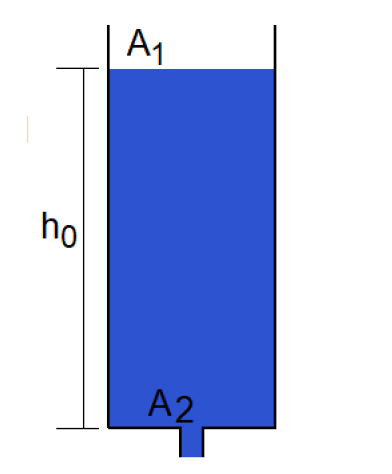
\includegraphics[width=0.5\textwidth]{img/esquema_tanque.png}
    \caption{Esquema de un tanque}
\end{figure}

Para ello, se realizó una maqueta utilizando un recipiente de plástico, cilíndrico y de un volumen entre 250 $cm^3$ a 2000 $cm^3$. Se realizaron mediciones para dos tipos de líquidos: agua coloreada (té) y un líquido más viscoso (aceite), utilizando distintos tamaños de orificios de salida. En este caso, al recipiente se le realizaron tres orificios de 4mm, 5mm y 6mm aproximadamente.

Se capturaron videos de cada una de las experiencias para poder tomar imágenes de distintos momentos y así medir las alturas de los líquidos en cada instante capturado. Para ello, se utilizó el programa ImageJ \footnote{\url https://imagej.net/software/fiji/downloads} para tomar los fotogramas a partir de los videos realizados. Una vez tomadas las distintas alturas, se confeccionaron tablas con las alturas y sus respectivos tiempos.

Por último, se realizaron distintos tipos de procesamiento numérico de datos, se analizaron y graficaron los resultados obtenidos.


\newpage
\section{Desarrollo}
A continuación se mostrará el desarrollo implementado durante este Trabajo Práctico

\subsection{Realización de la maqueta}
Como el recipiente se eligió un envase cilíndrico de aproximadamente 500 $cm^3$, al cual se le adhirió parte de una hoja milimetrada para tener referencias de distancias, y así poder tomar las alturas. La siguiente figura muestra la maqueta implementada:

\begin{figure}[H]
    \centering
    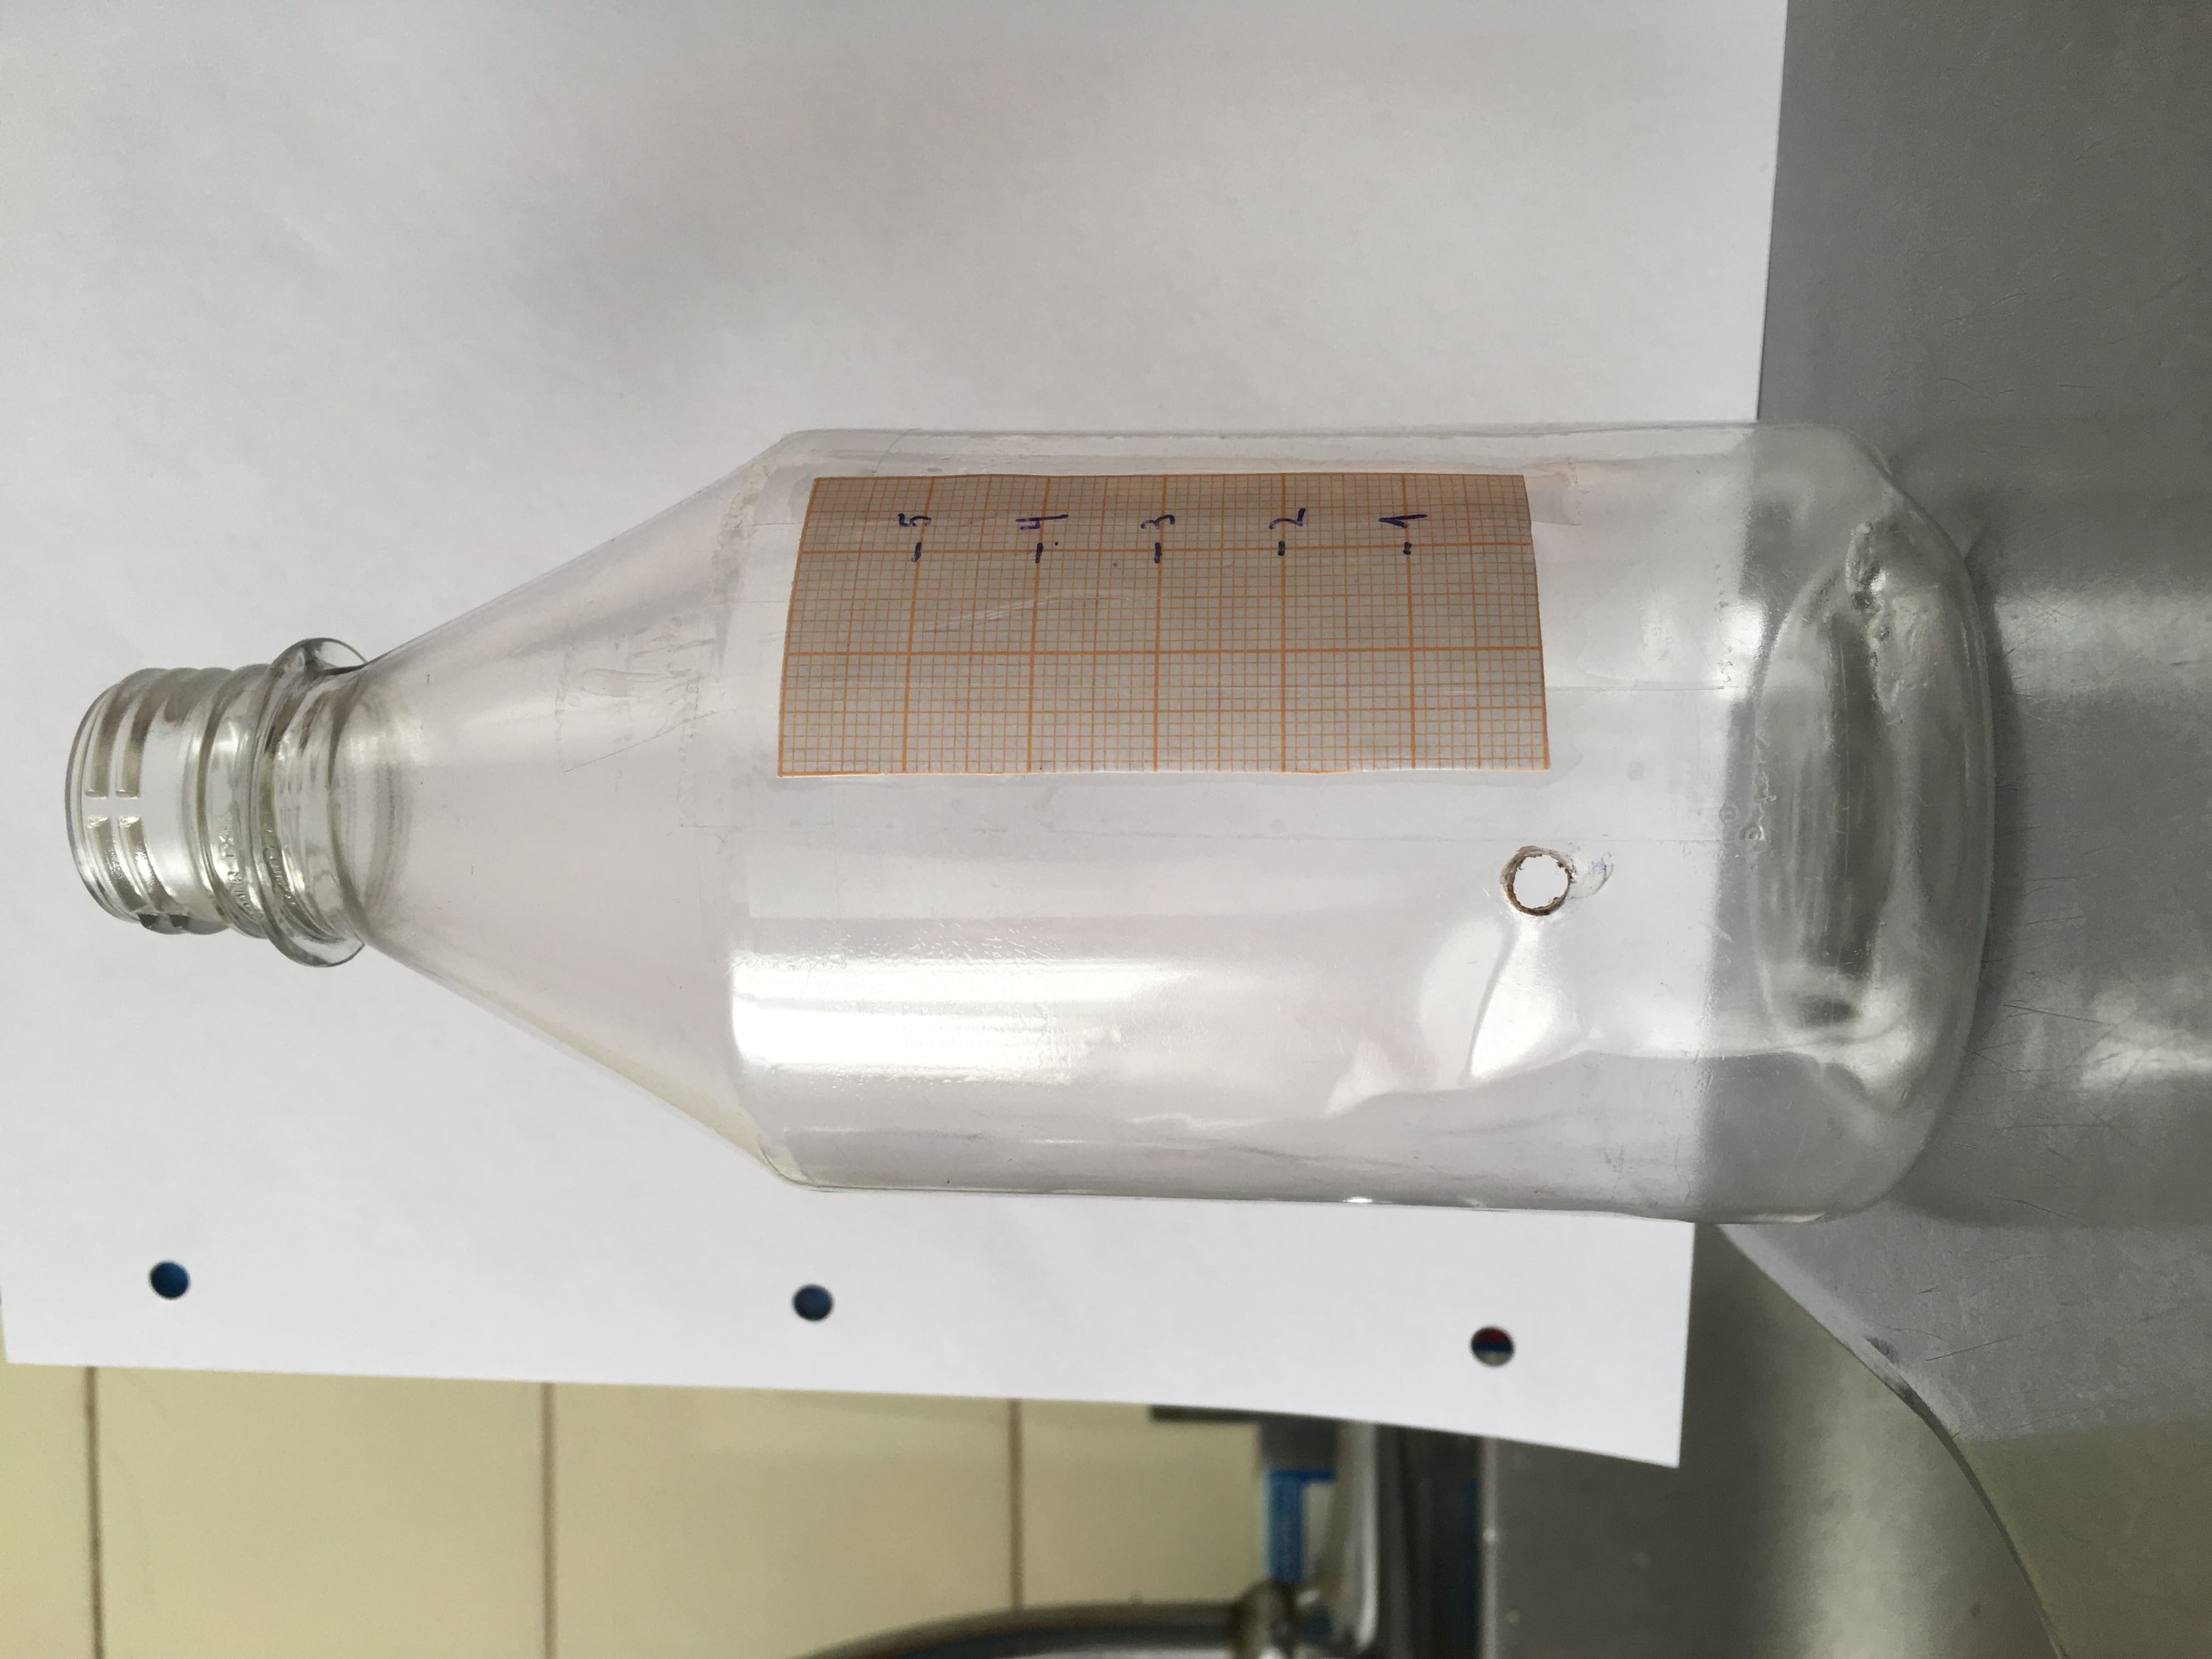
\includegraphics[width=0.8\textwidth, angle=270]{img/envase.JPG}
    \caption{Maqueta implementada}
\end{figure}

A continuación, se realizaron las mediciones para té y aceite para los distintos tamaños de orificios.

\subsection{Experiencias}

Para cada tamaño de agujero de salida se realizaron los mismos pasos que se describirán a continuación.

En primer lugar, se realizó el pequeño orificio en la parte inferior del envase. Como la base del envase no es horizontal, se colocó el agujero por arriba de la base y así tener una visión clara y uniforme de los líquidos. Con el fin de crear dicho agujero se utilizó un tornillo plano del diámetro deseado y se calentó la punta para poder realizar el orificio.

Para poder realizar las filmaciones, se posicionó la cámara o la cámara del celular en una posición fija y a una distancia del envase tal que sea visible con claridad el envase y la altura del líquido.  

Luego, se introdujo el agua coloreada tapando el orificio inferior para evitar que salga por allí, hasta una altura inicial medible por la hoja milimetrada y evitando que se generen burbujas en la película superior del líquido para poder observar con claridad y poder realizar las mediciones con el menor error posible. En la siguiente Figura se muestra como \textbf{NO} debe estar el liquido:    

\begin{figure}[H]
    \centering
    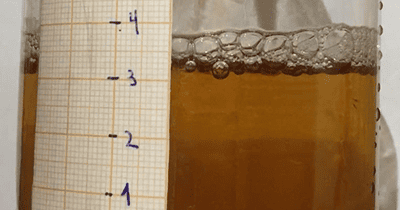
\includegraphics[width=0.5\textwidth]{img/burbujas.png}
    \caption{Envase MAL hecho con burbujas}
\end{figure}

Una vez llenado el recipiente se deja salir el líquido y se graba la experiencia hasta que deje de salir por el orificio o hasta que pase la medida de altura cero. En nuestro caso, se utilizó el nivel cero a la parte inferior de la hoja milimetrada, con el fin de tener una altura fija y sea más fácil la medición de la altura.

\begin{figure}[H]
    \centering
    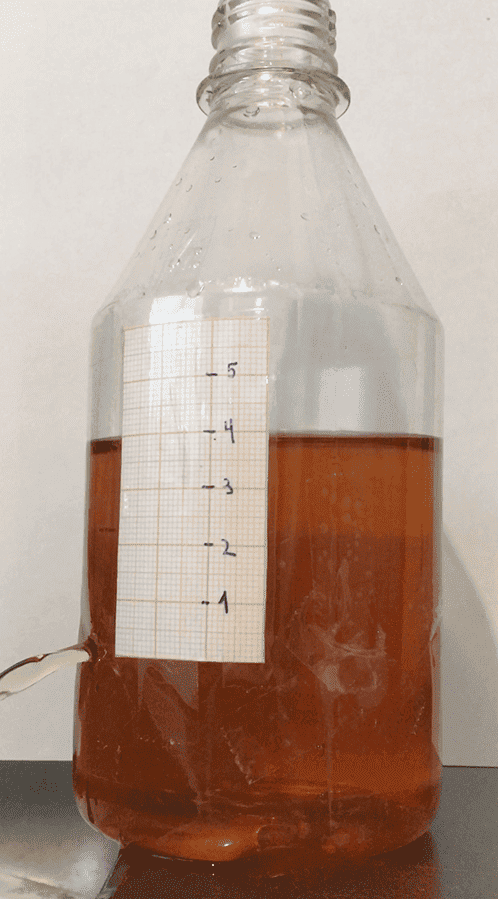
\includegraphics[width=0.5\textwidth]{img/te-saliendo.png}
    \caption{Experiencia Te}
\end{figure}

Al igual que con el agua coloreada, se llena el recipiente con aceite, se deja salir y se graba la experiencia hasta que deje de salir o hasta el nivel cero de altura.

\begin{figure}[H]
    \centering
    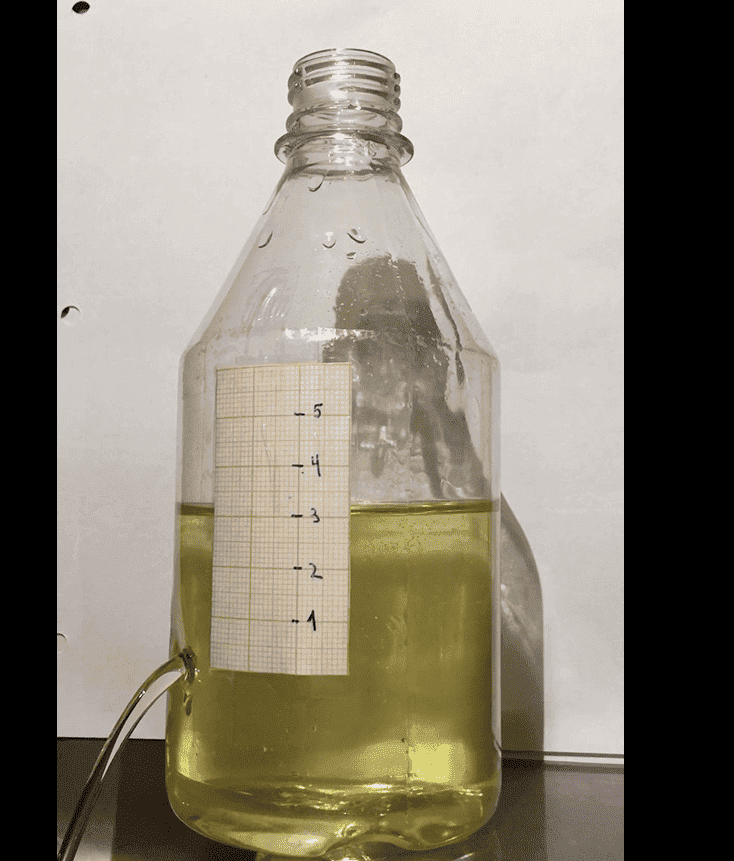
\includegraphics[width=0.5\textwidth]{img/aceite-saliendo.png}
    \caption{Experiencia Aceite}
\end{figure}

Al terminar las experiencias, se paso a la captura de los fotogramas para la realización de las mediciones.

\subsection{Captura de los fotogramas}
Como se mencionó en la Introducción, para la obtención de de los fotogramas se utilizó el programa ImageJ, el cual a partir de un video con la extensión .AVI, lo separa en imágenes con el tiempo de dicho momento.

Para ello, se capturaron 25 momentos a tiempos equidistantes, desde una altura inicial hasta que desagote o llegue al nivel de altura cero.

Para poder realizar correctamente las mediciones, se setea una escala en ImageJ para las imágenes. Usando la herramienta $Straight$ y la hoja milimetrada, tomamos una recta que mida aproximadamente 10mm. A partir de allí, en la sección Analyze, seleccionando Set Scale podemos crear una escala que relaciona pixeles con mm.  En la siguiente imagen se observa el seteo de una escala:

\begin{figure}[H]
    \centering
    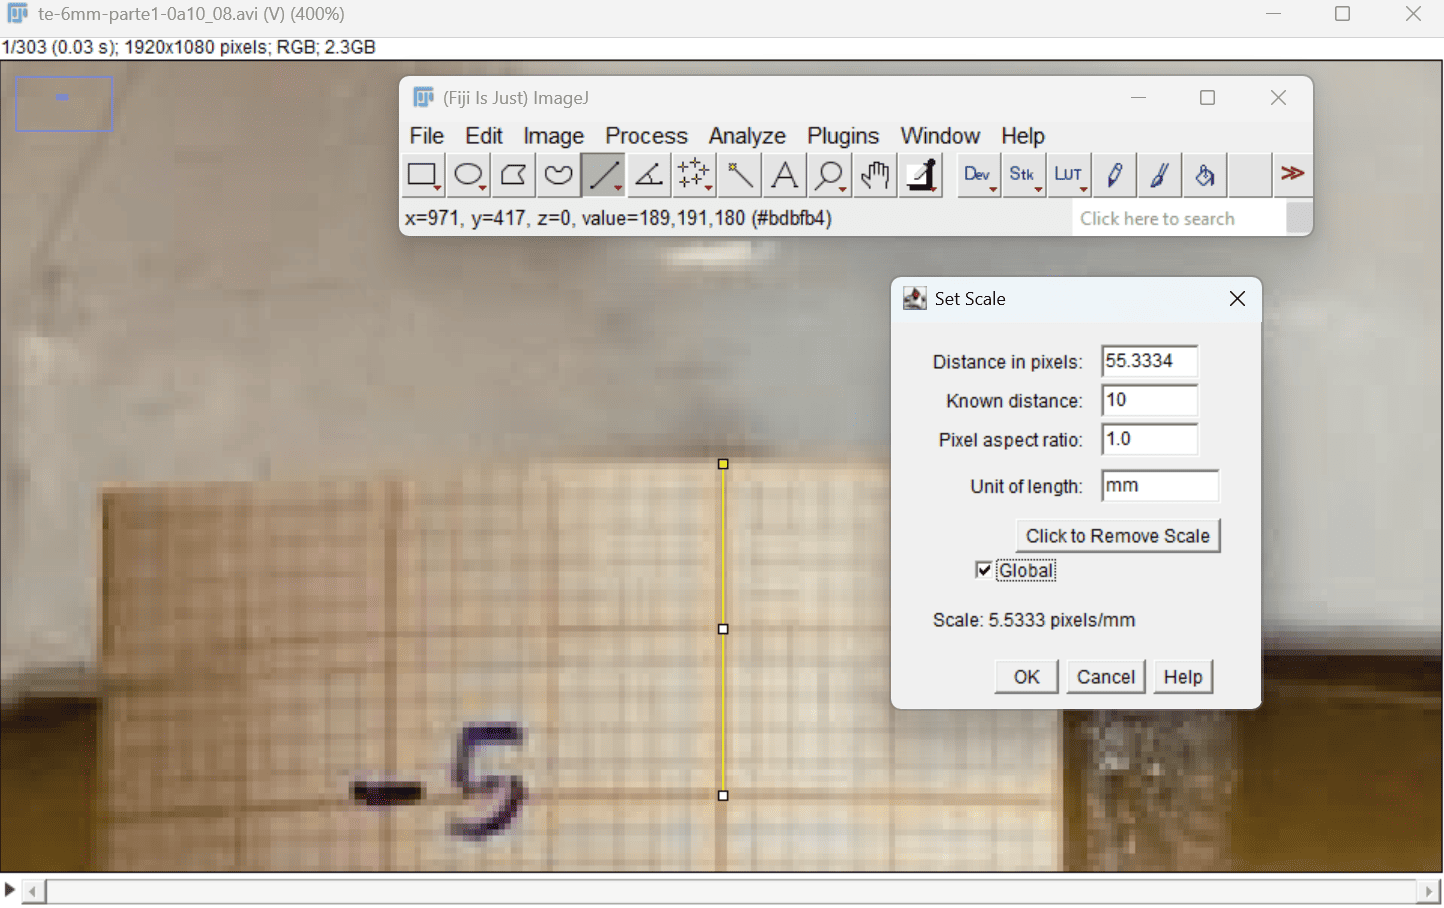
\includegraphics[width=0.9\textwidth]{img/set_scale_imagej.png}
    \caption{Ejemplo escala seteada con ImageJ}
\end{figure}

Como se observa en la imagen de ejemplo, nos indica que cada $5.5333$ pixeles equivale a 1 mm.

Utilizando la herramienta $Straight$ previamente mencionada, al apretar en la sección Analyze, y seleccionar Measure, se guardará la distancia que medimos con la linea recta. A continuación, un ejemplo:

\begin{figure}[H]
    \centering
    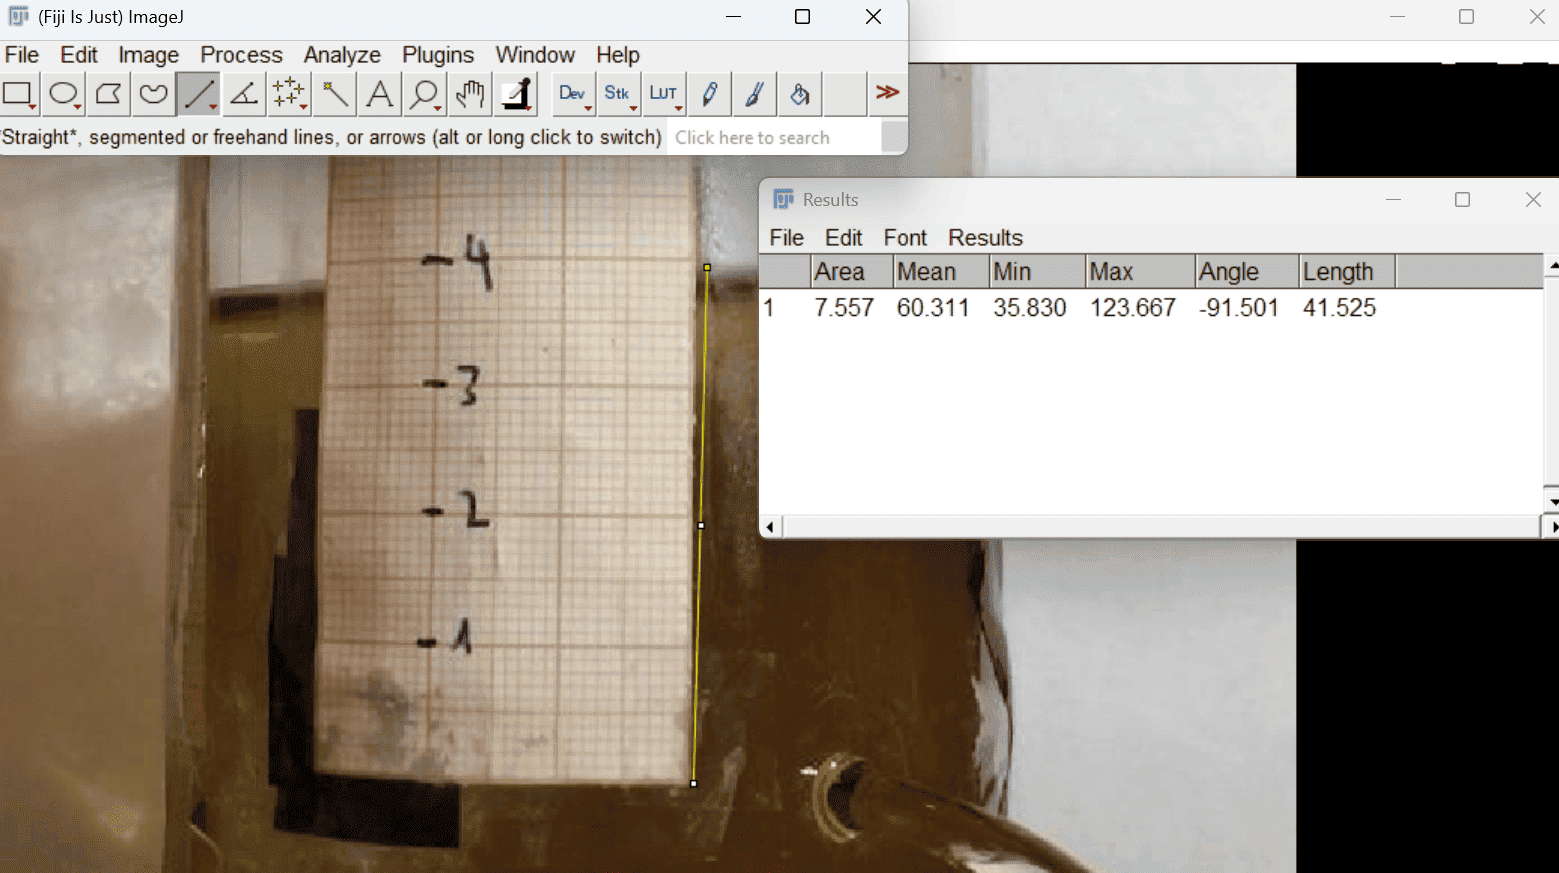
\includegraphics[width=0.9\textwidth]{img/medicion_altura.png}
    \caption{Ejemplo medición de una altura con ImageJ}
\end{figure}

En el ejemplo, podemos observar que la recta amarilla que seleccionamos equivale a $41.525$ mm

Al realizar estos pasos para los tres diámetros de agujeros y los 2 líquidos, obtendremos 6 tablas que relacionen el tiempo con la altura.

Para nuestro procesamiento numérico de datos, necesitaremos medir los diámetros de los orificios creados y de las secciones del envase. Para ello, utilizando las herramientas anteriormente mencionadas, mediremos los tamaños de dichos elementos. A continuación, un ejemplo:

\begin{figure}[H]
    \centering
    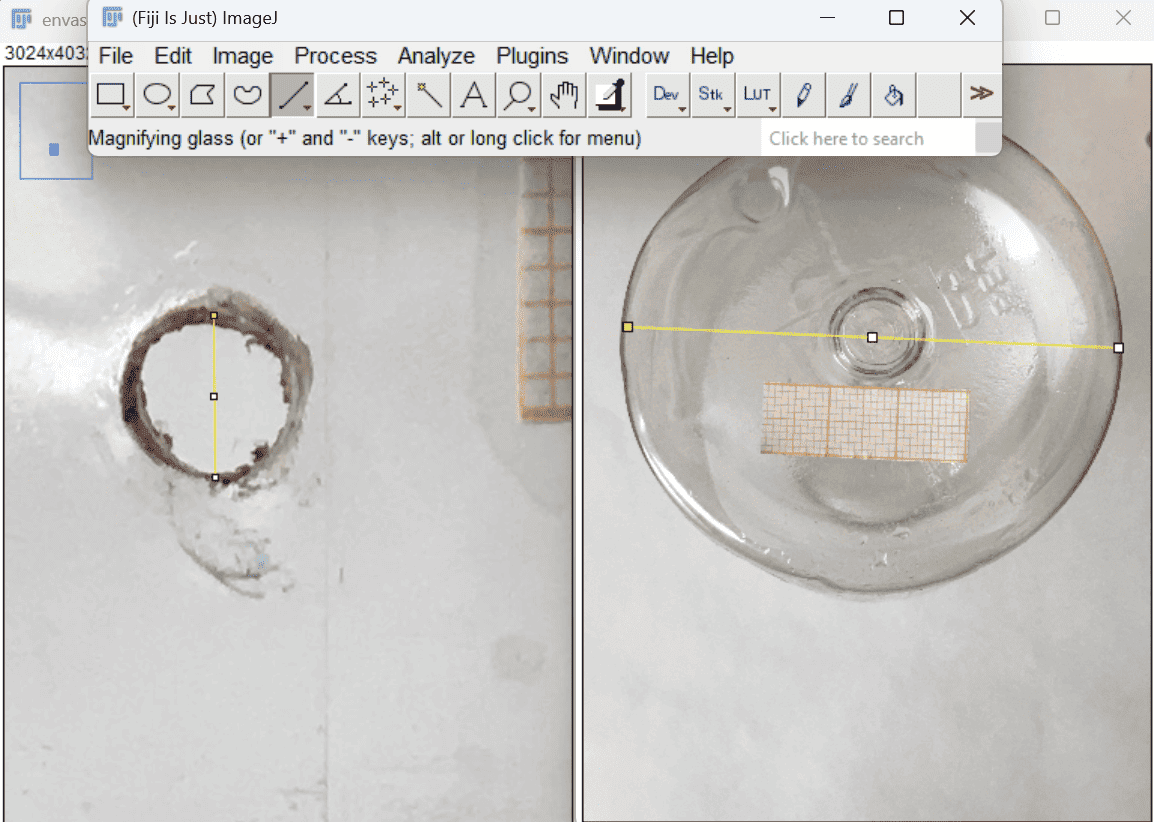
\includegraphics[width=0.9\textwidth]{img/orificio_base.png}
    \caption{Ejemplo medición del orificio y de la base con ImageJ}
\end{figure}

Con todos los datos y tablas obtenidas, realizamos procesamientos numéricos de datos, los analizamos y graficamos los datos. 


\subsubsection{Determinación de la cota de error de calibración}

Para estimar la incertidumbre de la calibración se midieron repetidamente
segmentos conocidos de la escala (1 cm y 1 mm) en distintas zonas y con
distintos zooms. 
Se constató que la
variación entre mediciones sucesivas es significativamente mayor que un
píxel, por lo que la precisión digital no refleja la precisión física de la escala.

En base a la variación observada y al grosor de las líneas milimetradas,
adoptamos como cota de error realista:
\[
\sigma_{\text{cal}} = 0.9\ \text{mm}.
\]

Esta cota se suma posteriormente en la propagación de errores de todas las
magnitudes geométricas.


\subsubsection{Estimación del diámetro y su incertidumbre}

Se realizaron al menos tres mediciones del
diámetro del orificio en distintos ángulos. Sea $D_i$ el conjunto de mediciones
obtenidas; definimos:
\[
\bar{D} = \frac{1}{n}\sum_i D_i,
\qquad
\Delta D = \frac{D_{\max} - D_{\min}}{2}.
\]

La incertidumbre total del diámetro resulta de sumar en cuadratura la cota de
error de calibración:
\[
\sigma_D = \sqrt{\Delta D^2 + \sigma_{\text{cal}}^2 }.
\]

Esta incertidumbre se propaga luego al área
\[
A = \frac{\pi D^2}{4},
\qquad
\sigma_{A} = \frac{\pi}{2} D\, \sigma_D.
\]

\subsubsection{Procesamiento de datos}

Con el fin de obtener un mejor análisis, se realizó un procesamiento de datos. 

Teniendo en cuenta la cota de error de calibración, decidimos descartar aquellas mediciones donde tengan mayor del 20\% de error, es decir, descartar los que sean del tipo $valores < cota\_calibracion * 5$. De esta manera nos aseguramos de tener mediciones claras. 

Luego del descarte, normalizamos las mediciones utilizando la primer altura.


\subsection{Métodos matemáticos}

Para poder analizar los datos, realizamos diferentes tipos de procesamientos numéricos y distintos tipos de cálculos matemáticos. Luego de los métodos matemáticos, se graficarán y compararán todos los resultados obtenidos. A continuación se enumerarán los cálculos realizados. 

\subsubsection{Ajustes por cuadrado mínimo}
En primer lugar, realizamos el ajuste por cuadrados mínimos para las alturas normalizadas $h(t)/h_0$ de la columna de líquido del tanque en función del tiempo utilizando tres modelos diferentes:

\begin{itemize}
    \item Modelo Cuadrático: $y = a + bt + ct^2$, con
    \begin{itemize}
        \item $cuad\_\phi_1 = 1$
        \item $cuad\_\phi_2 = t$
        \item $cuad\_\phi_3 = t^2$
    \end{itemize}
    \item Modelo Cúbico: $y = a + bt + ct^2 + dt^3$, con
    \begin{itemize}
        \item $cub\_\phi_1 = 1$
        \item $cub\_\phi_2 = t$
        \item $cub\_\phi_3 = t^2$
        \item $cub\_\phi_4 = t^3$
    \end{itemize}
    \item Modelo Exponencial: $y = e^{a-bt}$
\end{itemize}

Para el caso del Modelo Exponencial, linealizamos los datos, obteniendo una sumatoria de funciones lineales, y poder realizar el ajuste por cuadrados mínimos. Para ello, aplicamos logaritmo a ambos lados de la ecuación de la siguiente forma:
\begin{equation}
    y = e^{a-bt} \xrightarrow[]{} ln(y) = ln(e^{a-bt}) \xrightarrow[]{} ln(y) = ln(a) - bt
\end{equation}
obteniendo las siguientes funciones lineales:
\begin{center}
    \begin{minipage}{0.8\textwidth}
        \begin{itemize}
            \item $exp\_\phi_1 = ln(a)$
            \item $exp\_\phi_2 = t$
        \end{itemize}
    \end{minipage}
\end{center}

Para resolver los ajustes por cuadrados mínimos, se utilizaron las librerías Numpy y Matplotlib del lenguaje de programación Python, con el fin de poder calcular los coeficientes adecuados tal que minimicen el error cuadrático, y de esta manera obtener las funciones de dichos modelos. En la sección Segundo Anexo se mostrarán los códigos implementados. 

Además, se implementó un algoritmo que obtenga los coeficientes a través del esquema de resolución del método lineal de cuadrados mínimos expresado en forma matricial, de la siguiente forma $A*c = b$, donde:

\begin{enumerate}
    \item A es la matriz de los productos internos entre las funciones $\phi$
    \item c es la matriz de los coeficientes a calcular
    \item b es la matriz de los productos internos entre la función f y las funciones $\phi$
\end{enumerate}
de esta manera, poder comparar con los coeficientes obtenidos usando la función Polyfit de la librería Numpy. El algoritmo implementada se encuentra en el anexo Segundo Anexo

Para sumar otro elemento de análisis, se les calculo los Errores Cuadráticos Medios (ECM).

\subsubsection{Modelo Teórico}
Luego, se utilizó un modelo teórico donde la altura del líquido en función del tiempos se calcula con la siguiente ecuación:

\begin{equation}
    {h(t) = h_0 (1 -\frac{t}{t_f})^2}
    \tag{Ecuación 1}
\end{equation}

donde $t_f$ representa el tiempo de vaciado del tanque, el cual se puede representar de la siguiente manera:

\begin{equation}
    {t_f = \sqrt {2\frac{h_0}{g}(\frac{A_1^2}{A_2^2}-1)}}
    \tag{Ecuación 2}
\end{equation}

siendo $A_1$ el diámetro del envase y $A_2$ el diámetro del orificio de salida.

Ademas tenemos que agregar las respectivas cotas. En primer lugar tenemos la cota de error para $h(t)$, la cual se calcula de la siguiente forma:

\begin{equation}
    {\Delta h = \left|\frac{\delta h}{\delta h_0}\right|\Delta h_0 + \left|\frac{\delta h}{\delta t}\right|\Delta t + \left|\frac{\delta h}{\delta t_f}\right|\Delta t_f} \tag {Ecuación 3}
\end{equation}

teniendo la cotas de error para $h_0$, siendo la cota de error de calibración; la cota de error para t; y la cota de error para $t_f$

La cota de $t_f$, se calcula de la siguiente manera:

\begin{equation}
    {\Delta t_f = \left|\frac{\delta t_f}{\delta h_0}\right|\Delta h_0 + \left|\frac{\delta t_f}{\delta A_1}\right|\Delta A_1 + \left|\frac{\delta t_f}{\delta A_2}\right|\Delta A_2} \tag {Ecuación 4} 
\end{equation}

siendo $A_1$ el área del orificio del tanque y $A_2$ el área del orificio de salida. Ambas áreas y sus respectivas cotas se obtienen con las fórmulas mencionadas en la sección de \textbf{Estimación del diámetro y su incertidumbre}

Además para un tener un modelo que estime de la mejor manera, decidimos descartar las mediciones con tiempo mayor al tiempo final de vaciado obtenido por la Ecuación 2.

\subsubsection{Estimación del tiempo de vaciado del tanque}
Utilizando la Ecuación 1, se calculo el tiempo que se tarda en vaciar el $50\%$ del tanque y el $90\%$ del tanque. 
Para ello, a partir de la Ecuación 1 despejamos la variable t, obteniendo como resultado la siguiente ecuación:

\begin{equation}
    {t = t_f(1 \pm \sqrt{\frac{h(t)}{h_0}})}
    \tag{Ecuación 5}
\end{equation}

donde en este caso, conocemos los valores que tomará $h(t)$, que para el $50\%$ del tanque será $h(t) = 0.5*h_0$ y para el $90\%$ del tanque será $h(t) = 0.9*h_0$.

Además debemos calcularle la cota de error, usando la siguiente formula:

\begin{equation}
    {\Delta t = \left|\frac{\delta t}{\delta t_f}\right|\Delta t_f + \left|\frac{\delta t}{\delta h_0}\right|\Delta h_0} \tag {Ecuación 6} 
\end{equation}

siendo $\Delta t_f$ la cota de error de $t_f$ usando la Ecuación 4 mencionada anteriormente en esta sección.


Comparamos dichas estimaciones con el valor obtenido usando la expresión del ajuste cúbico. Y para ello, utilizamos el Método de Bisección para obtener el tiempo para cada vaciado teniendo el intervalo que contiene a nuestra raíz [$t_0 = 0.0$ y $t_f = t\_final$], siendo nuestra F(x) = 0 la siguiente:
\begin{equation}
    F(t) = h = a + bt + ct^2 + dt^3 \xrightarrow{} 0 = a - h + bt + ct^2 + dt^3
\end{equation}
además, para tener una cota de tres decimales, se realizaron 16 iteraciones
\begin{equation}
    \Delta_{16}=\frac{\Delta_0}{2^{16}}=\frac{b_0-a_0}{2^{16+1}} \leq 0.0005
\end{equation}
de esta manera, nuestros tiempos bien redondeados serán con tres decimales ($Ej: 18.12321344 \pm 0.0005 \xrightarrow{} 18.123 $).

\newpage
\section{Resultados}
En esta sección se mostrarán los datos obtenidos.

Se mostrarán algunas tablas con algunos valores, las tablas completas se encuentran en la sección Primer Anexo.

\subsection{Orificio de 4mm}
Usando ImageJ, se tomaron varias mediciones del diámetro del orificio y se promediaron, dando como resultado un diámetro de $4.069$ mm. Para el diámetro del envase, nos dio un promedio de $21.813$ mm
\subsubsection{Líquido usado: Té}
\begin{table}[h]
    \begin{center}
        \begin{tabular}{ | m{2cm} | m{2cm} | m{2cm} | }
            \hline N° medición & Tiempos (s) & Alturas (mm) \\ 
            \hline 1 & 0.03 & 54.680 \\
            \hline 2 & 1.80 & 50.471 \\
            \hline 3 & 3.57 & 46.249 \\
            \hline \vdots & \vdots & \vdots \\            
            \hline 23 & 38.90.32 & 4.792 \\
            \hline 24 & 40.67 & 4.397 \\
            \hline 25 & 42.43 & 4.052 \\
            \hline
        \end{tabular}
    \end{center}
    \caption{Tabla de alturas y tiempos para el líquido Té y orificio de 4mm}
\end{table}

\begin{table}[h]
    \begin{center}
        \begin{tabular}{ | m{2cm} | m{5cm} | m{2cm} | }
            \hline Modelo & Coeficientes & ECM \\ 
            \hline Cuadrático & \begin{itemize}
                \item a = 1.009
                \item b = -0.047
                \item c = 6.1e-4
            \end{itemize} & 1.851e-05 \\
            \hline Cúbico & \begin{itemize}
                \item a = 1.003
                \item b = -0.045
                \item c = 4.7e-4
                \item d = 2e-6
            \end{itemize} & 9.943e-06 \\
            \hline Exponencial & \begin{itemize}
                \item a = 0.116
                \item b = 0.068
            \end{itemize} & 1.223e-03 \\
            \hline
        \end{tabular}
    \end{center}
    \caption{Coeficientes obtenidos por Ajuste de cuadrados mínimos para el líquido Té y orificio de 4mm}
\end{table}

\begin{figure}[H]
    \centering
    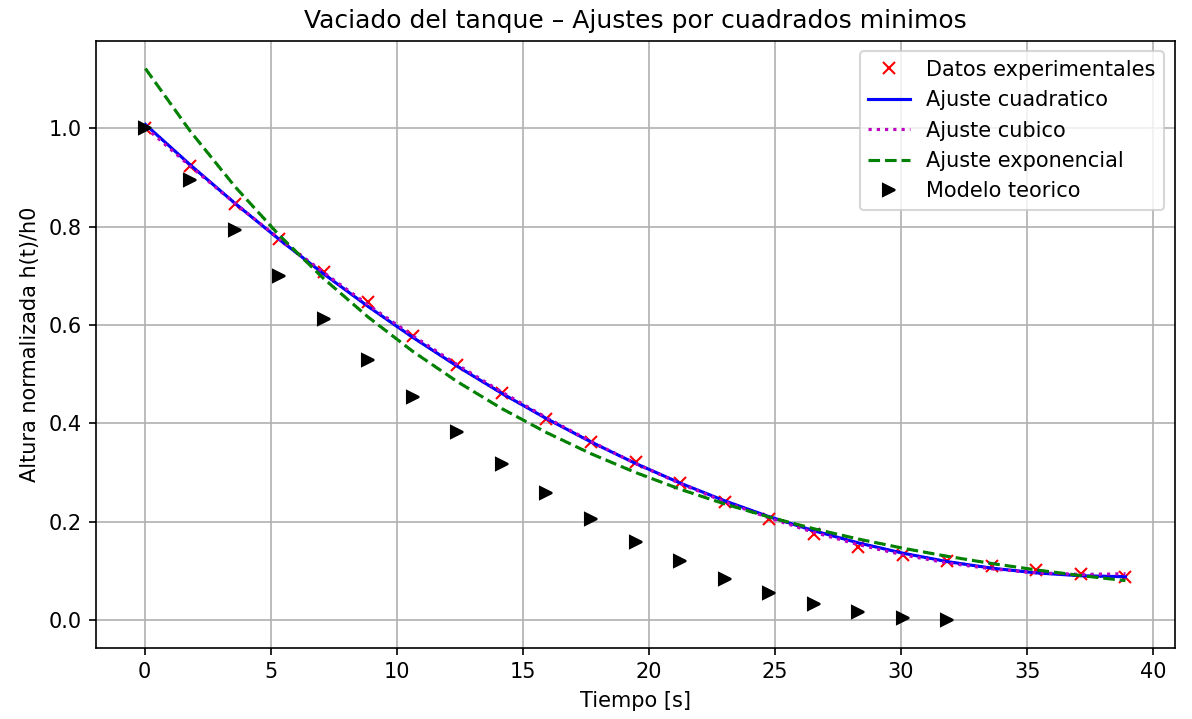
\includegraphics[width=0.93\textwidth]{img/ajuste_te_4mm.png}
    \caption{Gráfico de comparación de valores medidos y calculados para el líquido Té y orificio de 4mm}
\end{figure}

\begin{figure}[H]
    \centering
    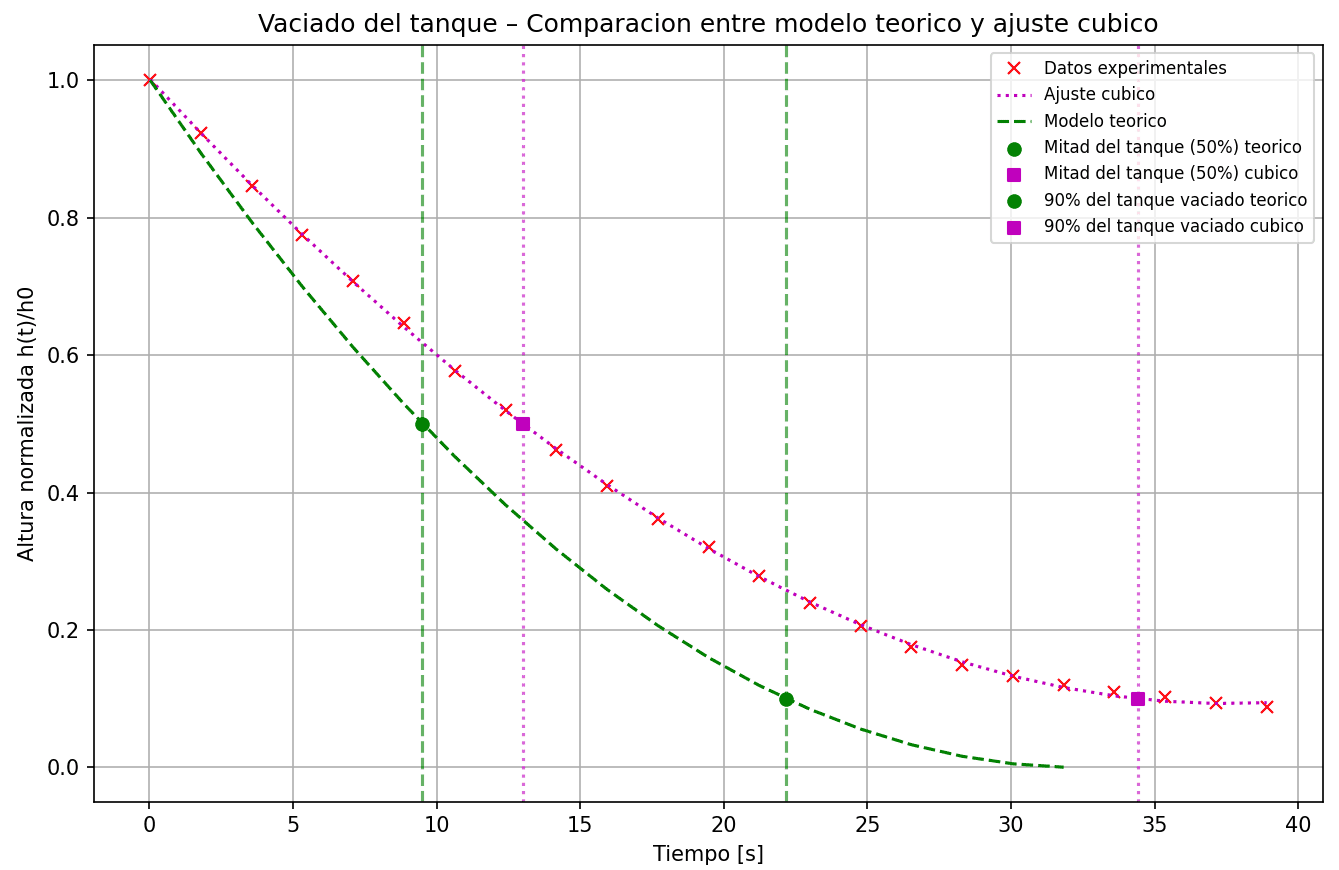
\includegraphics[width=0.93\textwidth]{img/tiempos_vaciado_te_4mm.png}
    \caption{Comparación entre los datos experimentales, el modelo teórico y el ajuste cúbico para el vaciado del té con orificio de 4 mm.
    Se muestran las curvas ajustadas junto con las líneas verticales que indican los tiempos teóricos y experimentales correspondientes al 50\% y al 90\% del vaciado del tanque.}
\end{figure}

\begin{table}[h]
    \centering
    \begin{center}
        \begin{tabular}{ | m{2cm} | m{2cm} | m{2cm} | m{2cm} | m{2cm} | }
            \hline Caso & t teórico (s) & dt teórico (s) & t cúbico (s) & dt cúbico (s) \\ 
            \hline 50\% tanque & 9.496 & 5.405 & 12.997 & 0.033 \\
            \hline 90\% tanque & 22.168 & 11.907 & 34.405 & 0.033 \\
            \hline
        \end{tabular}
    \end{center}
    \caption{Se observa que el modelo teórico predice correctamente el vaciado hasta aproximadamente la mitad del tanque, teniendo en cuenta la cota de error. Sin embargo, hacia el final del proceso el tiempo experimental resulta ligeramente mayor, debido a pequeñas pérdidas de carga y efectos de rozamiento en el orificio.}
\end{table}

\subsubsection{Líquido usado: Aceite}
\begin{table}[H]
    \begin{center}
        \begin{tabular}{ | m{2cm} | m{2cm} | m{2cm} | }
            \hline N° medición & Tiempos (s) & Alturas (mm) \\ 
            \hline 1 & 0.03 & 36.858 \\
            \hline 2 & 2.39 & 33.334 \\
            \hline 3 & 4.75 & 29.694 \\
            \hline \vdots & \vdots & \vdots \\            
            \hline 23 & 51.88 &  2.452\\
            \hline 24 & 54.24 & 2.138 \\
            \hline 25 & 56.60 & 1.872 \\
            \hline
        \end{tabular}
    \end{center}
    \caption{Tabla de alturas y tiempos para el líquido Aceite y orificio de 4mm}
\end{table}

\begin{table}[h]
    \begin{center}
        \begin{tabular}{ | m{2cm} | m{5cm} | m{2cm} | }
            \hline Modelo & Coeficientes & ECM \\ 
            \hline Cuadrático & \begin{itemize}
                \item a = 0.999
                \item b = -0.043
                \item c = 5.4e-4
            \end{itemize} & 1.987e-05 \\
            \hline Cúbico & \begin{itemize}
                \item a = 1.006
                \item b = -0.046
                \item c = 6.9e-4
                \item d = -3e-6
            \end{itemize} & 9.782e-06 \\
            \hline Exponencial & \begin{itemize}
                \item a = 0.059
                \item b = 0.057
            \end{itemize} & 2.964e-04 \\
            \hline
        \end{tabular}
    \end{center}
    \caption{Coeficientes obtenidos por Ajuste de cuadrados mínimos para el líquido Aceite y orificio de 4mm}
\end{table}

\begin{figure}[H]
    \centering
    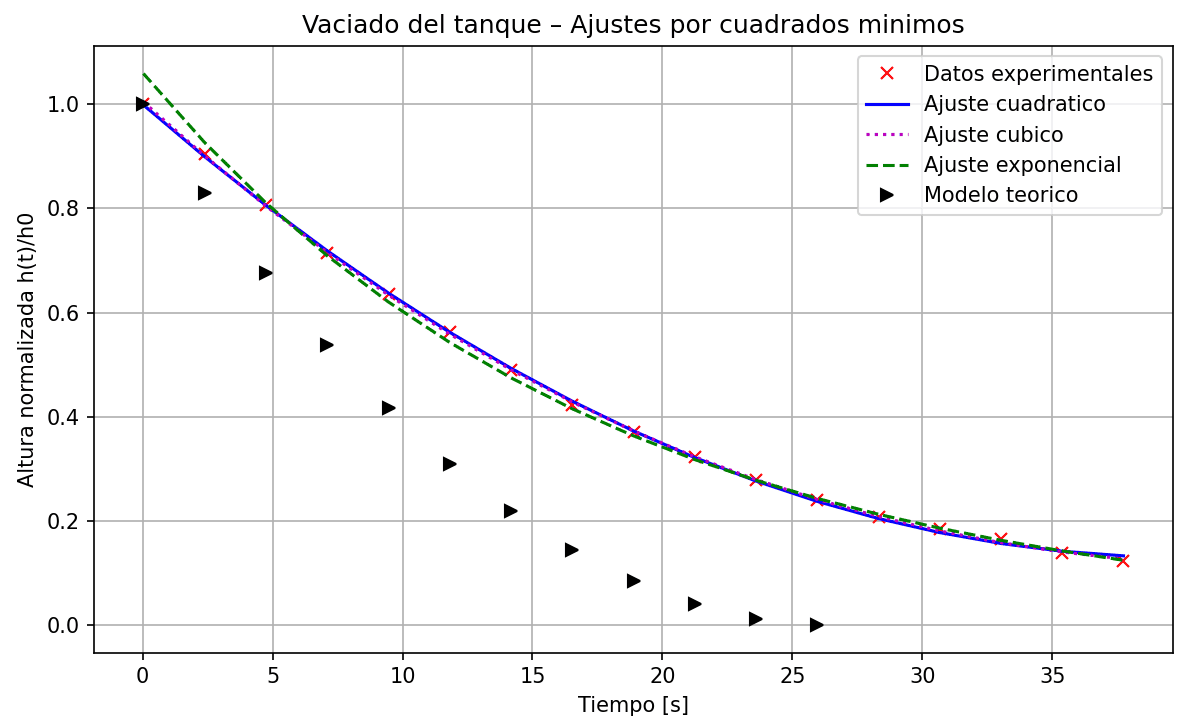
\includegraphics[width=0.93\textwidth]{img/ajuste_aceite_4mm.png}
    \caption{Gráfico de comparación de valores medidos y calculados para el líquido Aceite y orificio de 4mm}
\end{figure}

\begin{figure}[H]
    \centering
    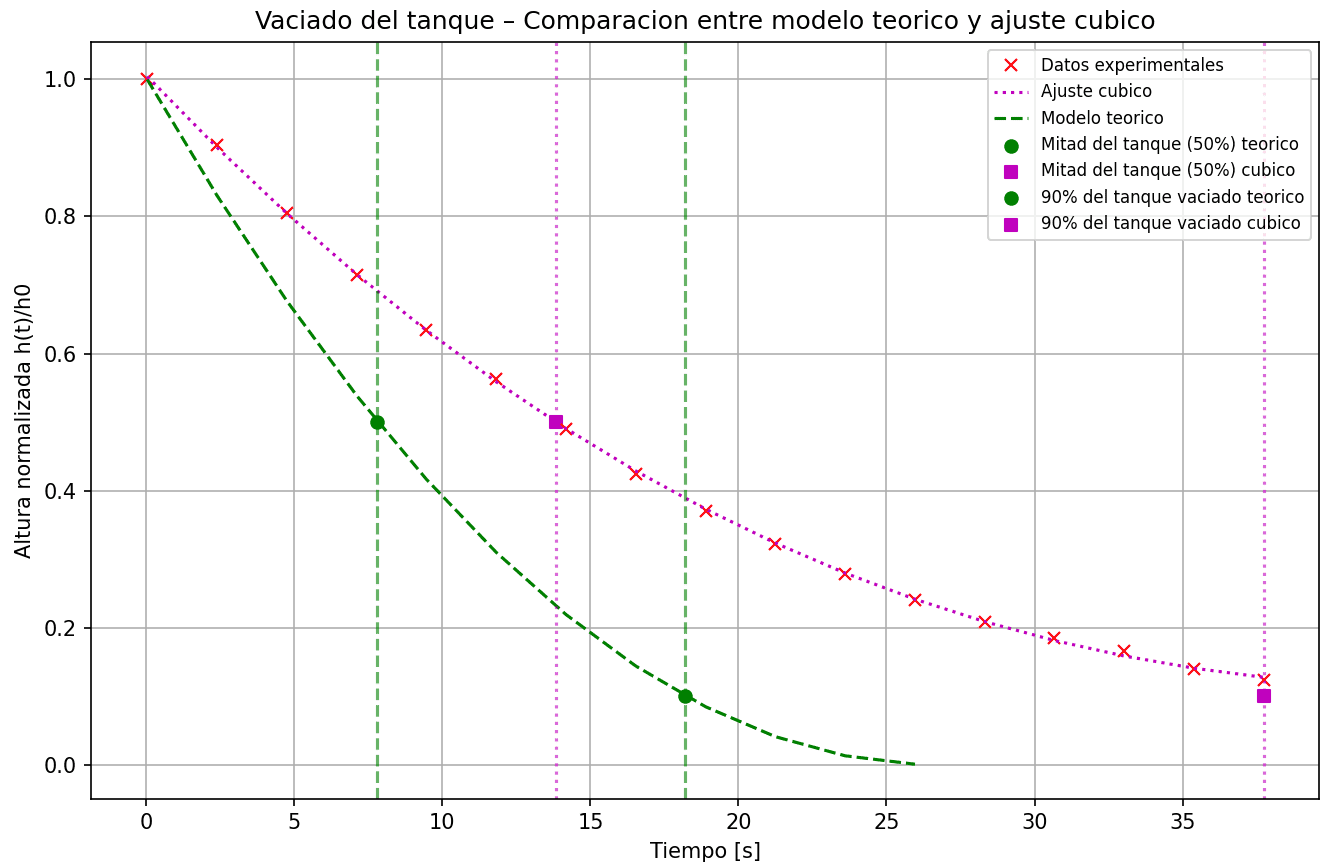
\includegraphics[width=0.93\textwidth]{img/tiempos_vaciado_aceite_4mm.png}
    \caption{Resultados del vaciado del aceite con orificio de 4 mm, comparando el modelo teórico y el ajuste cúbico.
    Se observan mayores desviaciones respecto a la teoría, especialmente hacia el final, debido a la viscosidad del fluido que reduce la velocidad de descarga y prolonga el tiempo total de vaciado.}
\end{figure}

\begin{table}[h]
    \centering
    \begin{center}
        \begin{tabular}{ | m{2cm} | m{2cm} | m{2cm} | m{2cm} | m{2cm} | }
            \hline Caso & t teórico (s) & dt teórico (s) & t cúbico (s) & dt cúbico (s) \\ 
            \hline 50\% tanque & 7.796 & 4.693 & 13.830 & 0.033 \\
            \hline 90\% tanque & 18.200 & 10.088 & 37.740 & 0.033 \\
            \hline
        \end{tabular}
    \end{center}
    \caption{En este caso, las diferencias entre el modelo teórico y los datos experimentales ya se pueden evidenciar incluso antes del 50\%, lo que refleja la influencia de la viscosidad del fluido. El aceite presenta mayor resistencia al flujo y un vaciado más lento que el previsto por la ecuación ideal.}
\end{table}

\subsection{Orificio de 5mm}
Usando ImageJ, se tomaron varias mediciones del diámetro del orificio y se promediaron, dando como resultado un diámetro de $5.071$ mm. Para el diámetro del envase, nos dio un promedio de $21.813$ mm
\subsubsection{Líquido usado: Té}
\begin{table}[h]
    \begin{center}
        \begin{tabular}{ | m{2cm} | m{2cm} | m{2cm} | }
            \hline N° medición & Tiempos (s) & Alturas (mm) \\ 
            \hline 1 & 0.05 & 56.991 \\
            \hline 2 & 1.23 & 51.525 \\
            \hline 3 & 2.41 & 48.059 \\
            \hline \vdots & \vdots & \vdots \\            
            \hline 23 & 26.07 & 4.199 \\
            \hline 24 & 27.26 & 3.811 \\
            \hline 25 & 28.44 & 3.495 \\
            \hline
        \end{tabular}
    \end{center}
    \caption{Tabla de alturas y tiempos para el líquido Té y orificio de 5mm}
\end{table}

\begin{table}[h]
    \begin{center}
        \begin{tabular}{ | m{2cm} | m{5cm} | m{2cm} | }
            \hline Modelo & Coeficientes & ECM \\ 
            \hline Cuadrático & \begin{itemize}
                \item a = 1.011
                \item b = -0.073
                \item c = 0.001
            \end{itemize} & 1.361e-05 \\
            \hline Cúbico & \begin{itemize}
                \item a = 1.005
                \item b = -0.070
                \item c = 0.001
                \item d = -9e-6
            \end{itemize} & 5.782e-06 \\
            \hline Exponencial & \begin{itemize}
                \item a = 0.149
                \item b = 0.110
            \end{itemize} & 1.967e-03 \\
            \hline
        \end{tabular}
    \end{center}
    \caption{Coeficientes obtenidos por Ajuste de cuadrados mínimos para el líquido Té y orificio de 5mm}
\end{table}

\begin{figure}[H]
    \centering
    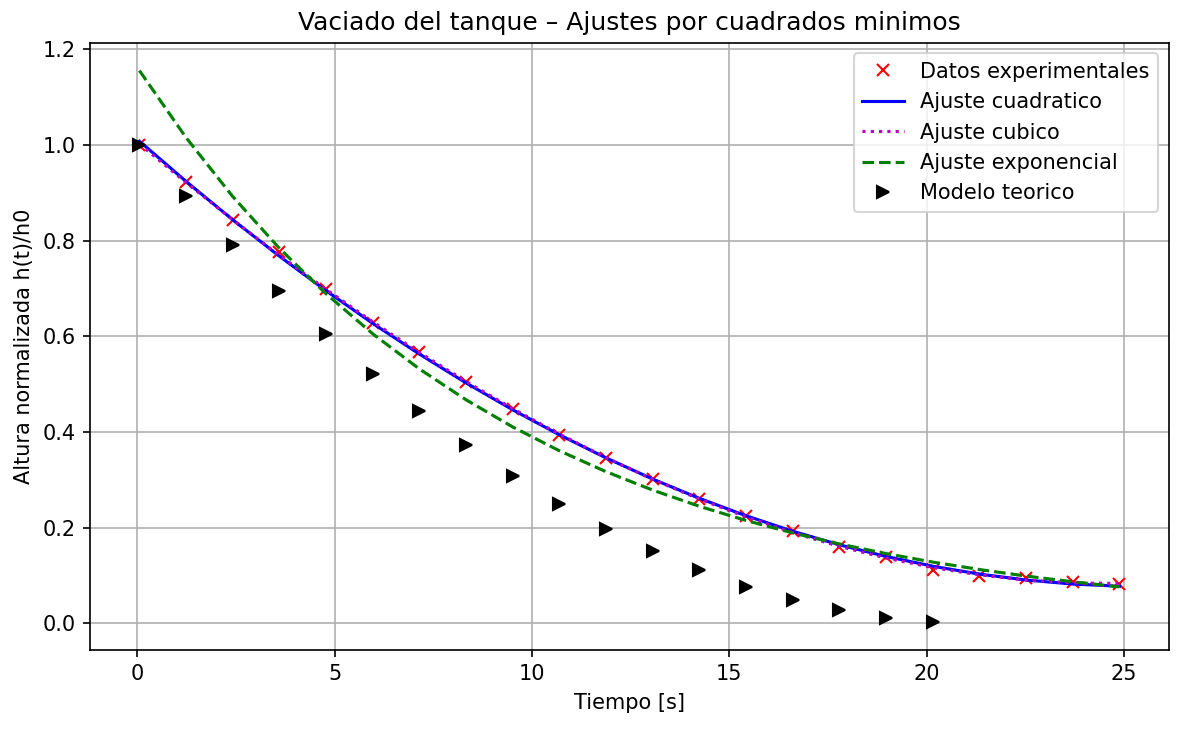
\includegraphics[width=0.93\textwidth]{img/ajuste_te_5mm.png}
    \caption{Gráfico de comparación de valores medidos y calculados para el líquido Té y orificio de 5mm}
\end{figure}

\begin{figure}[H]
    \centering
    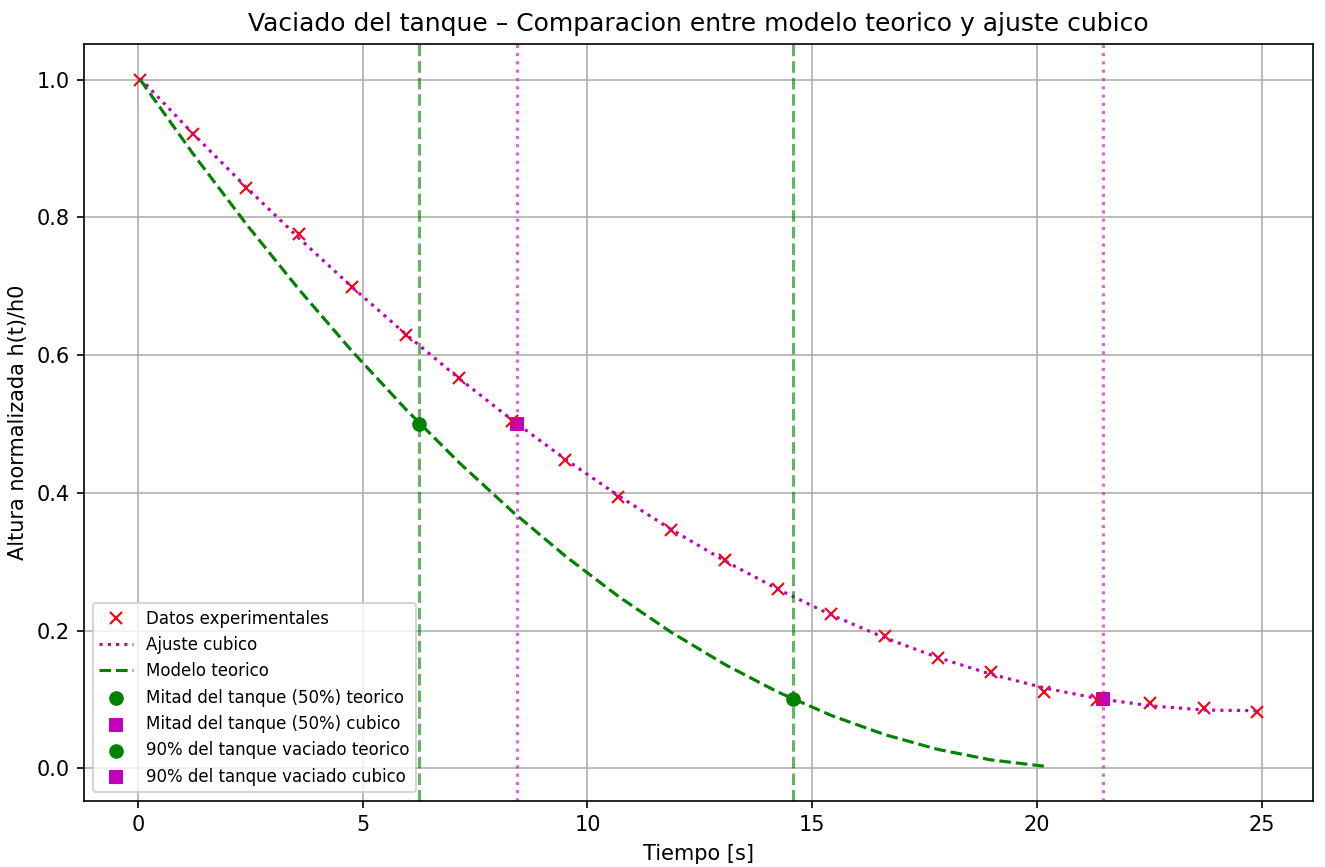
\includegraphics[width=0.93\textwidth]{img/tiempos_vaciado_te_5mm.png}
    \caption{Comparación entre los datos experimentales, el modelo teórico y el ajuste cúbico para el vaciado del té con orificio de 5 mm.
Las líneas verdes y violetas marcan los tiempos teóricos y experimentales de vaciado al 50\% y al 90\% de la altura inicial.
El modelo teórico predice un poco mejor, aunque el tiempo experimental al final resulta mayor debido a efectos de fricción y turbulencia en el orificio.}
\end{figure}

\begin{table}[h]
    \centering
    \begin{center}
        \begin{tabular}{ | m{2cm} | m{2cm} | m{2cm} | m{2cm} | m{2cm} | }
            \hline Caso & t teórico (s) & dt teórico (s) & t cúbico (s) & dt cúbico (s) \\ 
            \hline 50\% tanque & 6.242 & 2.993 & 8.440 & 0.033 \\
            \hline 90\% tanque & 14.571 & 6.538 & 21.468 & 0.033 \\
            \hline
        \end{tabular}
    \end{center}
    \caption{El modelo teórico reproduce muy bien el comportamiento teniendo en cuenta las cotas de error para el vaciado de 50\% y 90\%. Sin embargo, se observa como el modelo experimental es mucho mas lento. Esto se atribuye principalmente a pérdidas de energía y a la menor precisión de medición en la parte final del vaciado.}
\end{table}

\subsubsection{Líquido usado: Aceite}

\begin{table}[H]
    \begin{center}
        \begin{tabular}{ | m{2cm} | m{2cm} | m{2cm} | }
            \hline N° medición & Tiempos (s) & Alturas (mm) \\ 
            \hline 1 & 0.03 & 52.797 \\
            \hline 2 & 1.32 & 48.455 \\
            \hline 3 & 2.61 & 44.124 \\
            \hline \vdots & \vdots & \vdots \\            
            \hline 23 & 28.41 & 3.491 \\
            \hline 24 & 29.70 & 3.103 \\
            \hline 25 & 30.99 & 2.879 \\
            \hline
        \end{tabular}
    \end{center}
    \caption{Tabla de alturas y tiempos para el líquido Aceite y orificio de 5mm}
\end{table}

\begin{table}[h]
    \begin{center}
        \begin{tabular}{ | m{2cm} | m{5cm} | m{2cm} | }
            \hline Modelo & Coeficientes & ECM \\ 
            \hline Cuadrático & \begin{itemize}
                \item a = 1.006
                \item b = -0.068
                \item c = 0.001
            \end{itemize} & 2.335e-05 \\
            \hline Cúbico & \begin{itemize}
                \item a = 1.001
                \item b = -0.065
                \item c = 0.001
                \item d = 9e-6
            \end{itemize} & 1.752e-05 \\
            \hline Exponencial & \begin{itemize}
                \item a = 0.146
                \item b = 0.103
            \end{itemize} & 2.270e-03 \\
            \hline
        \end{tabular}
    \end{center}
    \caption{Coeficientes obtenidos por Ajuste de cuadrados mínimos para el líquido Aceite y orificio de 5mm}
\end{table}

\begin{figure}[H]
    \centering
    
\includegraphics[width=0.93\textwidth]{img/ajuste_aceite_5mm.png}
    \caption{Gráfico de comparación de valores medidos y calculados para el líquido Aceite y orificio de 5mm}
\end{figure}

\begin{figure}[H]
    \centering
    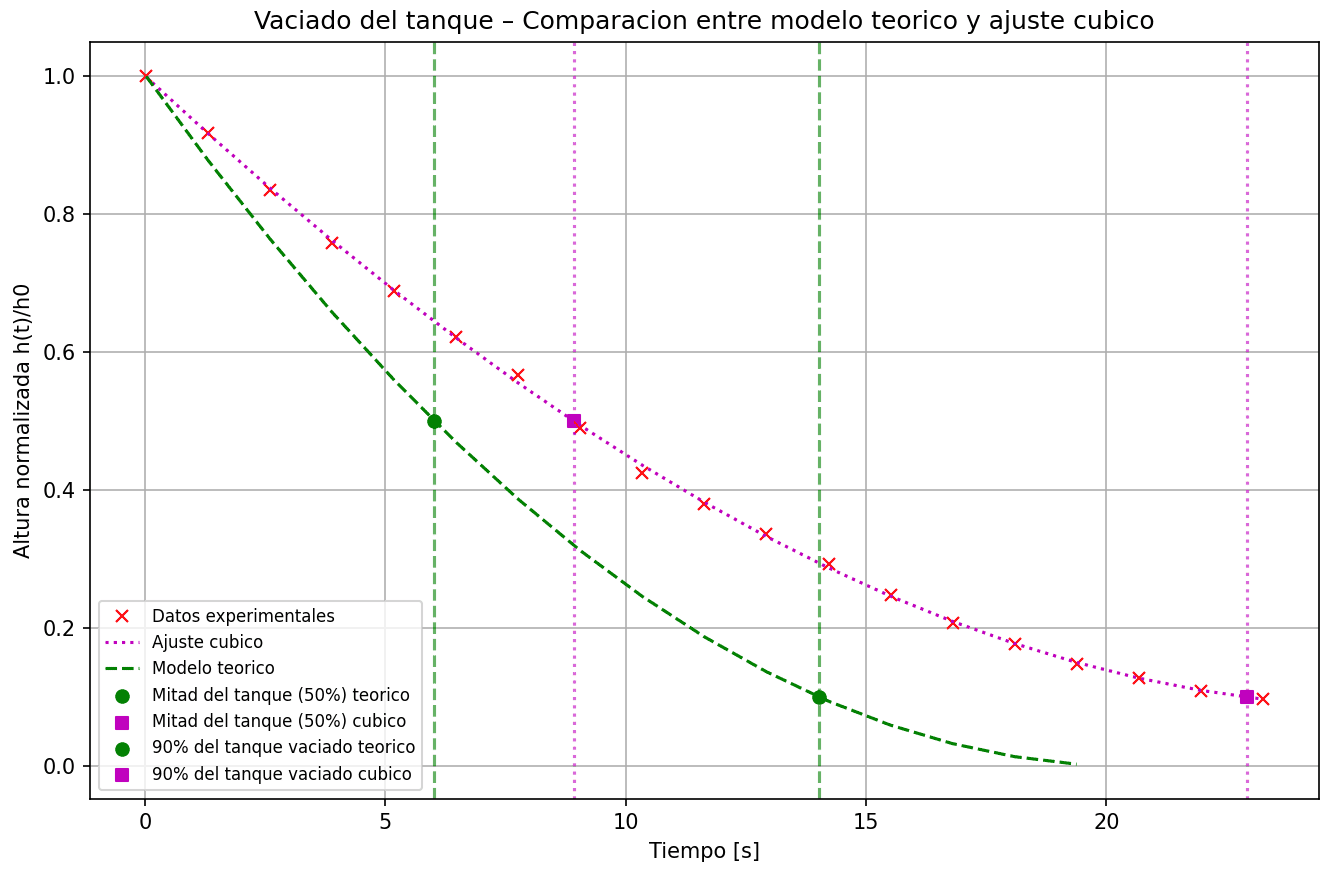
\includegraphics[width=0.93\textwidth]{img/tiempos_vaciado_aceite_5mm.png}
    \caption{Comparación entre el modelo teórico y el ajuste cúbico para el vaciado del aceite con orificio de 5 mm.
    El comportamiento experimental muestra un vaciado más lento que el predicho por la ecuación ideal.}
\end{figure}

\begin{table}[h]
    \centering
    \begin{center}
        \begin{tabular}{ | m{2cm} | m{2cm} | m{2cm} | m{2cm} | m{2cm} | }
            \hline Caso & t teórico (s) & dt teórico (s) & t cúbico (s) & dt cúbico (s) \\ 
            \hline 50\% tanque & 6.008 & 2.913 & 8.929 & 0.033 \\
            \hline 90\% tanque & 14.025 & 6.335 & 22.932 & 0.033 \\
            \hline
        \end{tabular}
    \end{center}
    \caption{Se observa que el modelo teórico predice correctamente el vaciado hasta aproximadamente la mitad del tanque, pero para el 90\% del vaciado el tiempo experimental resulta mayor incluso considerando la cota de error, indicando que la descarga real es más lenta debido a los efectos de viscosidad y fricción.}
\end{table}

\subsection{Orificio de 6mm}

Usando ImageJ, se tomaron varias mediciones del diámetro del orificio y se promediaron, dando como resultado un diámetro de $5.982$ mm. Para el diámetro del envase, nos dio un promedio de $21.813$ mm

\subsubsection{Líquido usado: Té}
\begin{table}[h]
    \begin{center}
        \begin{tabular}{ | m{2cm} | m{2cm} | m{2cm} | }
            \hline N° medición & Tiempos (s) & Alturas (mm) \\ 
            \hline 1 & 0.03 & 57.163 \\
            \hline 2 & 1.33 & 52.163 \\
            \hline 3 & 2.64 & 46.487 \\
            \hline \vdots & \vdots & \vdots \\            
            \hline 23 & 28.66 & 0.947 \\
            \hline 24 & 29.96 & 0.766 \\
            \hline 25 & 31.26 & 0.676 \\
            \hline
        \end{tabular}
    \end{center}
    \caption{Tabla de alturas y tiempos para el líquido Té y orificio de 6mm}
\end{table}

\begin{table}[h]
    \begin{center}
        \begin{tabular}{ | m{2cm} | m{5cm} | m{2cm} | }
            \hline Modelo & Coeficientes & ECM \\ 
            \hline Cuadrático & \begin{itemize}
                \item a = 1.007
                \item b = -0.074
                \item c = 0.001
            \end{itemize} & 3.479e-05\\
            \hline Cúbico & \begin{itemize}
                \item a = 1.001
                \item b = -0.069
                \item c = 5.9e-4
                \item d = 2.6e-5
            \end{itemize} & 2.191e-05 \\
            \hline Exponencial & \begin{itemize}
                \item a = 0.183
                \item b = 0.124
            \end{itemize} & 4.411e-03 \\
            \hline
        \end{tabular}
    \end{center}
    \caption{Coeficientes obtenidos por Ajuste de cuadrados mínimos para el líquido Té y orificio de 6mm}
\end{table}

\begin{figure}[H]
    \centering
    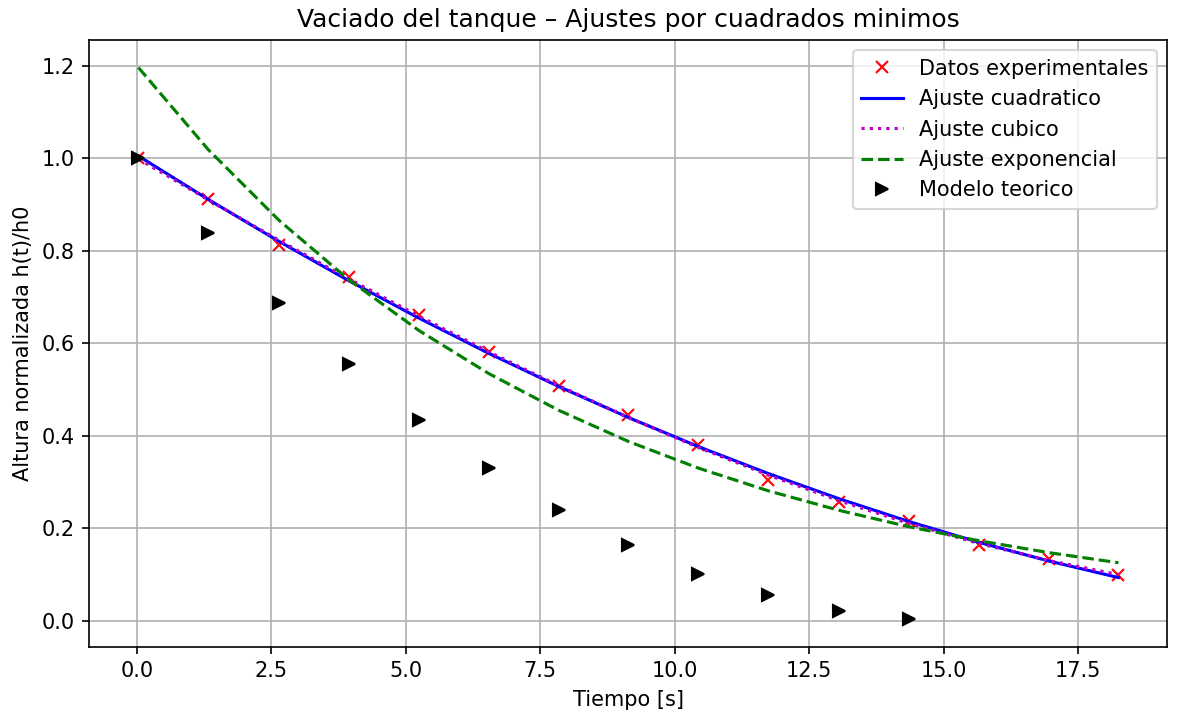
\includegraphics[width=0.93\textwidth]{img/ajuste_te_6mm.png}
    \caption{Gráfico de comparación de valores medidos y calculados para el líquido Té y orificio de 6mm}
\end{figure}

\begin{figure}[H]
    \centering
    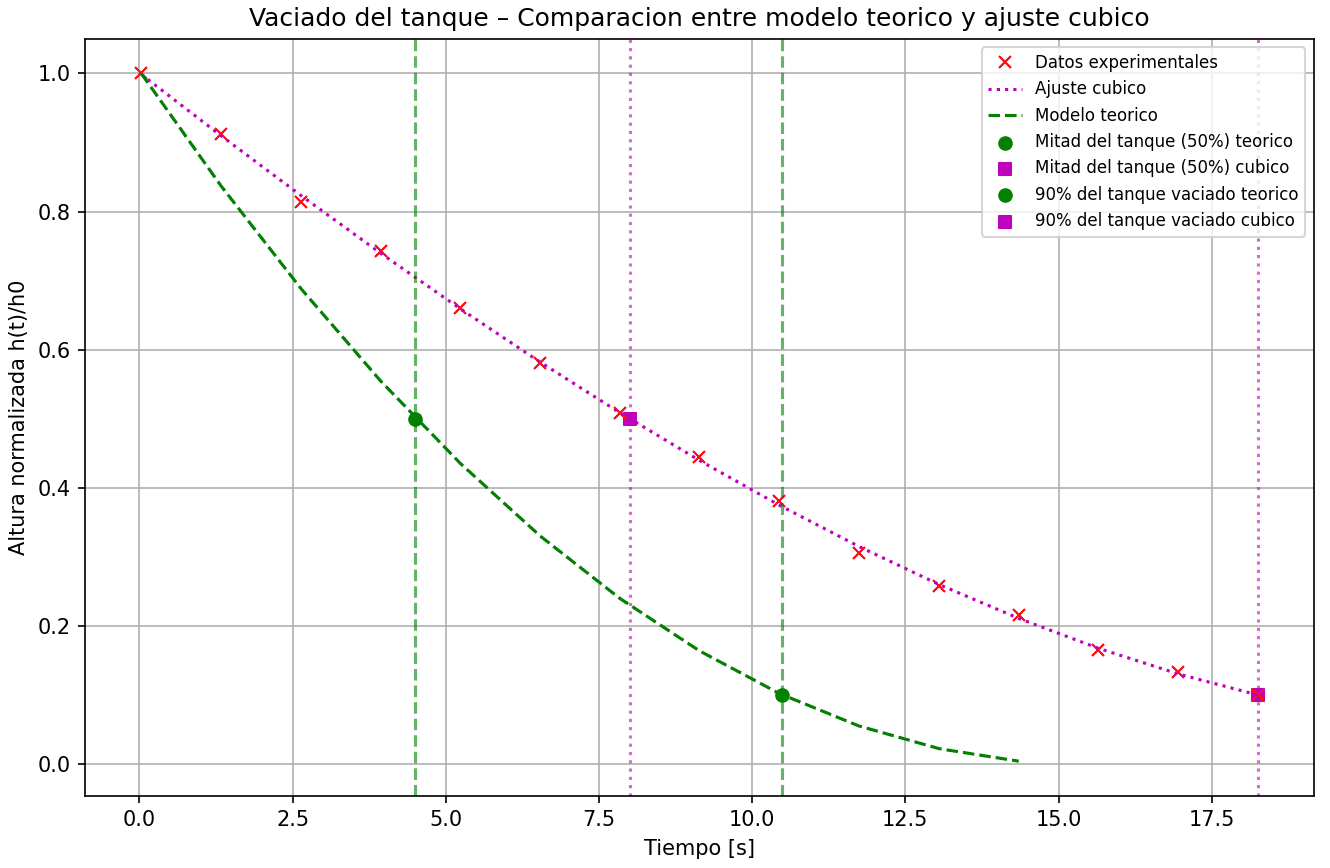
\includegraphics[width=0.93\textwidth]{img/tiempos_vaciado_te_6mm.png}
    \caption{Comparación entre el modelo teórico y el ajuste cúbico para el vaciado del te con orificio de 6 mm.
    El comportamiento teórico es mucho mas rápido que el experimental, algo que ocurre porque no tiene en cuenta la fricción, la turbulencia y el rozamiento del líquido.}
\end{figure}

\begin{table}[h]
    \centering
    \begin{center}
        \begin{tabular}{ | m{2cm} | m{2cm} | m{2cm} | m{2cm} | m{2cm} | }
            \hline Caso & t teórico (s) & dt teórico (s) & t cúbico (s) & dt cúbico (s) \\ 
            \hline 50\% tanque & 4.492 & 1.913 & 8.000 & 0.033 \\
            \hline 90\% tanque & 10.487 & 4.144 & 18.250 & 0.033 \\
            \hline
        \end{tabular}
    \end{center}
    \caption{Se observa que el modelo teórico tiende a ser 4seg aproximadamente mas rápido que el modelo experimental.}
\end{table}

\subsubsection{Líquido usado: Aceite}
\begin{table}[H]
    \begin{center}
        \begin{tabular}{ | m{2cm} | m{2cm} | m{2cm} | }
            \hline N° medición & Tiempos (s) & Alturas (mm) \\ 
            \hline 1 & 0.03 & 41.532 \\
            \hline 2 & 1.27 & 37.867 \\
            \hline 3 & 2.50 & 33.586 \\
            \hline \vdots & \vdots & \vdots \\            
            \hline 23 & 27.19 & 0.605 \\
            \hline 24 & 28.43 & 0.488 \\
            \hline 25 & 29.66 & 0.336 \\
            \hline
        \end{tabular}
    \end{center}
    \caption{Tabla de alturas y tiempos para el líquido Aceite y orificio de 6mm}
\end{table}

\begin{table}[h]
    \begin{center}
        \begin{tabular}{ | m{2cm} | m{5cm} | m{2cm} | }
            \hline Modelo & Coeficientes & ECM \\ 
            \hline Cuadrático & \begin{itemize}
                \item a = 1.006
                \item b = -0.081
                \item c = 0.002
            \end{itemize} & 1.605e-05 \\
            \hline Cúbico & \begin{itemize}
                \item a = 1.004
                \item b = -0.08
                \item c = 0.002
                \item d = 9e-6
            \end{itemize} & 1.487e-05\\
            \hline Exponencial & \begin{itemize}
                \item a = 0.148
                \item b = 0.125
            \end{itemize} & 2.641e-03\\
            \hline
        \end{tabular}
    \end{center}
    \caption{Coeficientes obtenidos por Ajuste de cuadrados mínimos para el líquido Aceite y orificio de 6mm}
\end{table}

\begin{figure}[H]
    \centering
    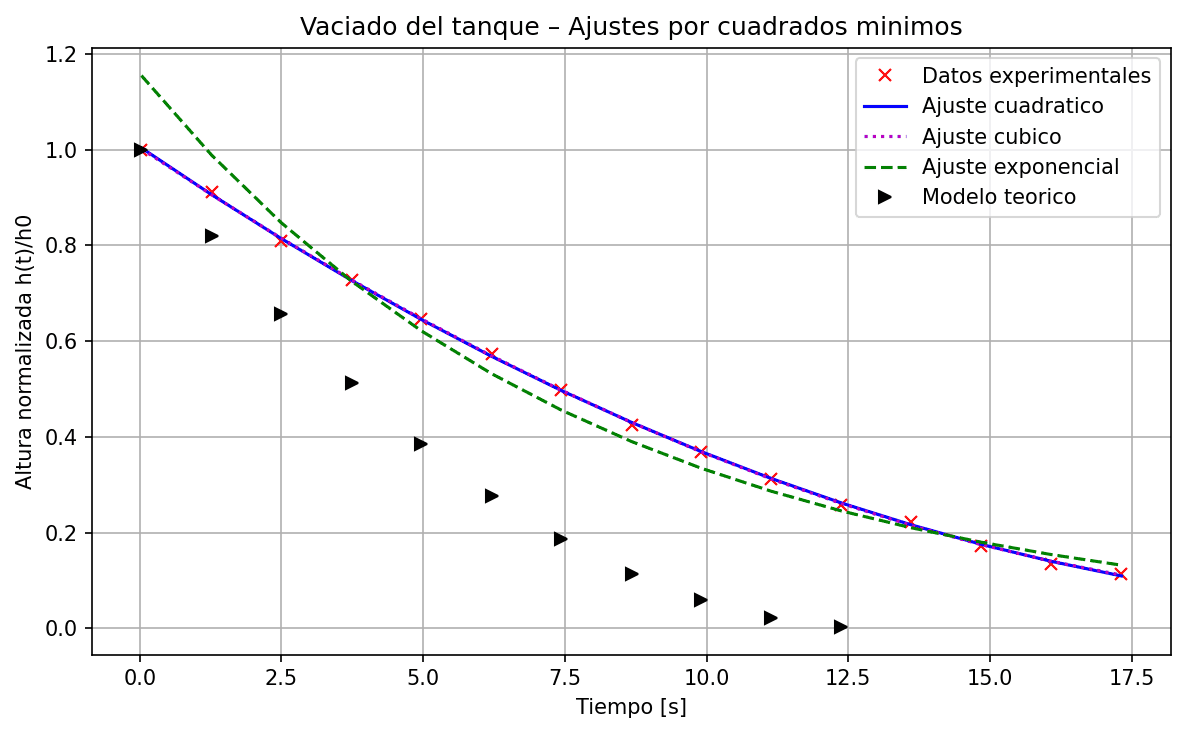
\includegraphics[width=0.93\textwidth]{img/ajuste_aceite_6mm.png}
    \caption{Gráfico de comparación de valores medidos y calculados para el líquido Aceite y orificio de 6mm}
\end{figure}

\begin{figure}[H]
    \centering
    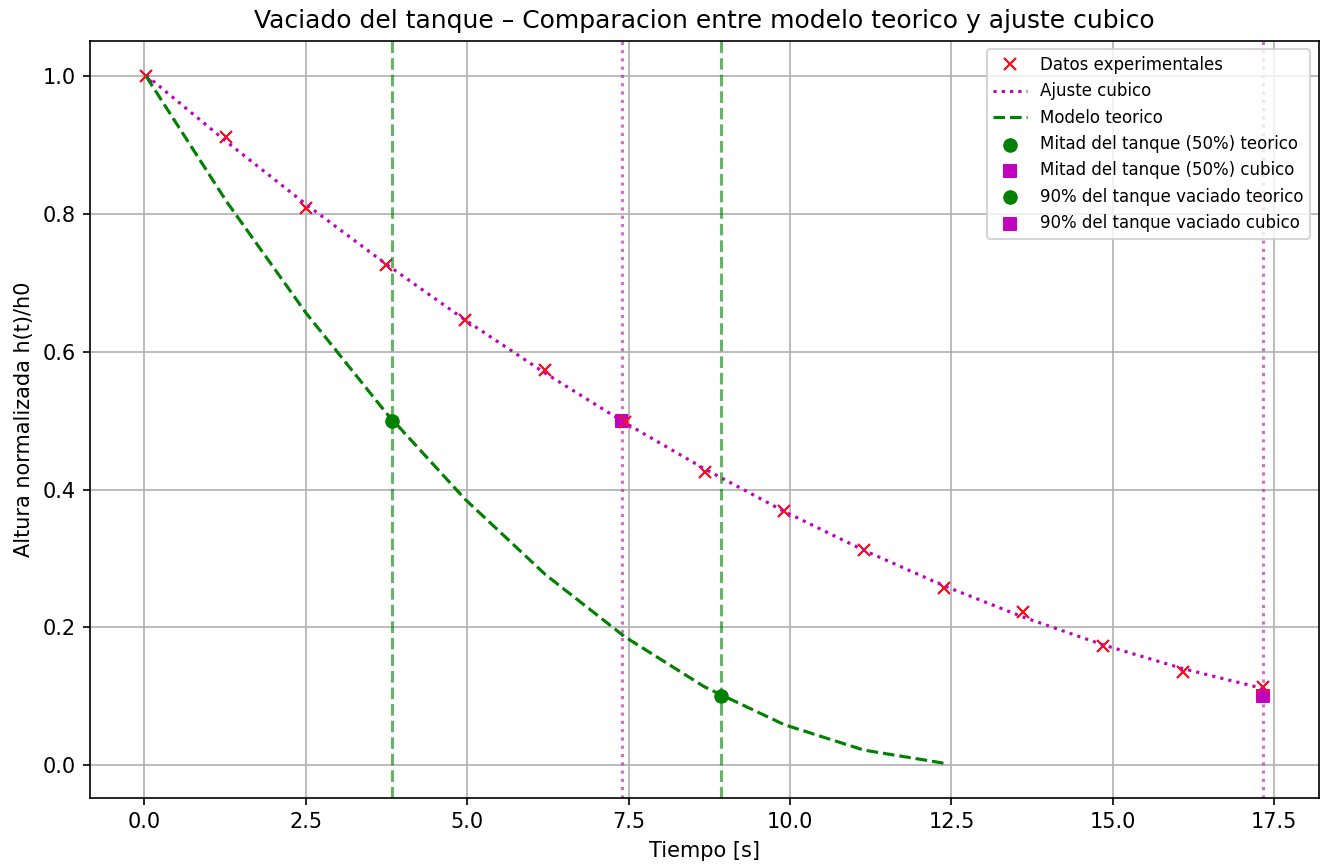
\includegraphics[width=0.93\textwidth]{img/tiempos_vaciado_aceite_6mm.png}
    \caption{Comparación entre el modelo teórico y el ajuste cúbico para el vaciado del aceite con orificio de 6 mm.
    El modelo teórico es mucho más rápido que el modelo experimental.}
\end{figure}

\begin{table}[H]
    \centering
    \begin{center}
        \begin{tabular}{ | m{2cm} | m{2cm} | m{2cm} | m{2cm} | m{2cm} | }
            \hline Caso & t teórico (s) & dt teórico (s) & t cúbico (s) & dt cúbico (s) \\ 
            \hline 50\% tanque & 3.829 & 1.726 & 7.392 & 0.033 \\
            \hline 90\% tanque & 8.939 & 3.652 & 17.320 & 0.033 \\
            \hline
        \end{tabular}
    \end{center}
    \caption{Se observa una gran diferencia entre el modelo teórico y el experimental. Se puede deber a la viscosidad del líquido y la fricción del mismo con el envase.}
\end{table}


\newpage
\section{Discusión de resultados}

La comparación entre los modelos teóricos y los datos experimentales permitió evaluar la validez de la ecuación de Torricelli para el vaciado de un tanque bajo distintas condiciones.
En general, los resultados muestran que el modelo teórico tiende a ser mucho más rápido que cualquier modelo experimental, haciendo que la tendencia del vaciado sea más rápido. En muy pocos casos, teniendo en cuenta la cota de error del modelo teórico, se puede ver una similitud con los valores del modelo experimental.

En todos los casos analizados, el ajuste cúbico fue el que presentó el menor error cuadrático medio (ECM), lo que indica que describe de forma más precisa la variación de la altura normalizada respecto al tiempo.
El ajuste cuadrático también se comportó razonablemente bien, mientras que el modelo exponencial fue el que peor representó la descarga del fluido, evidenciando que el proceso no responde a un decaimiento de tipo exponencial sino a una relación polinómica.

En cuanto al tamaño del orificio, se observó que el tiempo total de vaciado disminuye al aumentar el diámetro.
Esto coincide con la ecuación teórica, que predice una dependencia inversa entre el área del orificio y el tiempo de vaciado total.
Sin embargo, las discrepancias entre la teoría y los datos se acentúan para los orificios más grandes (6 mm), donde la fricción con las paredes, las pérdidas locales en la salida y la fluctuación del líquido afectan más el flujo.

El análisis del tipo de líquido confirma el rol de la viscosidad en la dinámica de descarga.
Mientras que el té (de comportamiento similar al agua) se aproxima al modelo ideal, el aceite muestra tiempos de vaciado significativamente mayores.
Esto se debe a que las pérdidas energéticas por fricción interna son más relevantes, lo que retrasa la salida del fluido, especialmente en la etapa final, cuando la velocidad es baja y el régimen de flujo se aleja del ideal.

En la estimación de los tiempos de vaciado parcial (50\% y 90\%), en la mayoria de los casos, el modelo teórico fu mucho más rapido que el ajuste cúbico. A medida que se aumentaba el tamaño del orificio de salida, mayor era la diferenicia. El líquido experimental tarda más en vaciarse de lo que predice la ecuación ideal, lo que puede atribuirse a la viscosidad, tensión superficial, aire atrapado en el orificio.
Estos efectos no están contemplados en la ecuación teórica, que supone flujo perfecto y sin pérdidas.

Por último, es importante destacar que la incertidumbre de medición y la propagación de los errores en la ecuación teórica del cálculo del tiempo aumenta hacia el final del proceso, ya que los cambios de altura son pequeños y el margen de error en la lectura de imágenes (±1 píxel o ±1 frame) se vuelve proporcionalmente más significativo.
Este efecto también contribuye a las diferencias observadas entre el modelo teórico y los valores experimentales del 90\%.

En síntesis, el modelo teórico describe adecuadamente el comportamiento global del vaciado para líquidos de baja viscosidad y en las etapas iniciales y medias del proceso.
Las desviaciones observadas en la parte final reflejan la influencia de fenómenos reales no ideales, como la fricción viscosa y las pérdidas locales, confirmando la necesidad de introducir correcciones empíricas o modelos de flujo no ideal para reproducir con precisión el comportamiento completo.

\subsubsection{Comparación con resultados de la primer entrega}

En comparación a los resultados obtenidos en la primer entrega, vemos que antes el modelo teórico se comportaba de manera similar al modelo cúbico en la mayoría de las experiencias, mientras que ahora el modelo teórico es mucho más rápido que el modelo experimental.

En cuanto al ECM, ahora se obtuvieron valores menores en comparación a la primer entrega.

A la hora de calcular el tiempo para el vaciado de 50\%, vemos que se obtuvieron tiempos menores en comparación a la primer entrega en todas las experiencias. Sin embargo, para el vaciado del 90\%, se obtuvieron valores similares a los de la primer entrega. Además, ahora se propagaron los errores y se obtuvo una cota de error mayor a la primer entrega. 

En conclusión, se bajaron los tiempos y se obtuvieron mejores métricas. El modelo teórico estima mucho más rápido que cualquier otro modelo, y el modelo cúbico sigue siendo el mejor de los otros modelos. 

\newpage
\section{Bibliografía}

\begin{enumerate}
    \item Página Oficial ImageJ, \url{https://imagej.net/ij/index.html}
    \item 30/8/25, Tutorial como pasar .MOV a .AVI en ImageJ, \url{https://www.youtube.com/watch?v=X29zKkvKwEk}
    \item 30/8/25, Tutorial como medir en ImageJ, \url{https://www.youtube.com/watch?v=2IruFzYUH80}
    \item OpenAI. (2025). Respuesta generada por ChatGPT a un prompt personalizado sobre la extracción de 25 fotogramas equidistantes en ImageJ. ChatGPT (versión GPT-5) [Modelo de lenguaje grande]. Recuperado de \url{https://chat.openai.com/}
    \item Osorio Joaquin (30/9/2025). Prompt utilizado en ChatGPT para solicitar instrucciones sobre cómo dividir un video en 25 momentos equidistantes en ImageJ: “Necesito obtener una serie de pasos detallados para dividir un video en 25 momentos equidistantes utilizando el programa ImageJ. El objetivo es extraer 25 fotogramas igualmente espaciados a lo largo de la duración total del video, de manera que cada imagen represente un instante uniforme del proceso. Por favor, explícame de forma clara y ordenada qué herramientas o comandos debo usar dentro de ImageJ, cómo abrir el video, cómo definir la cantidad de cuadros, entre otros.” ChatGPT (versión GPT-5) [Prompt de usuario].
\end{enumerate}




\newpage
\section{Primer anexo}
\subsection{Mediciones orificio 4 mm}

\subsubsection{Líquido usado: Te}
\begin{table}[H]
    \begin{center}
        \begin{tabular}{ | m{2cm} | m{2cm} | m{2cm} | }
            \hline N° medición & Tiempos (s) & Alturas (mm) \\ 
            \hline 1 & 0.03 & 54.680 \\
            \hline 2 & 1.80 & 50.471 \\
            \hline 3 & 3.57 & 46.249 \\
            \hline 4 & 5.33 & 42.392 \\
            \hline 5 & 7.10 & 38.723 \\
            \hline 6 & 8.87 & 35.390 \\
            \hline 7 & 10.63 & 31.538 \\
            \hline 8 & 12.40 & 28.409 \\
            \hline 9 & 14.17 & 25.279 \\
            \hline 10 & 15.93 & 22.360 \\
            \hline 11 & 17.70 & 19.784 \\
            \hline 12 & 19.47 & 17.570 \\
            \hline 13 & 21.23 & 15.253 \\
            \hline 14 & 23.00 & 13.112 \\
            \hline 15 & 24.77 & 11.242 \\
            \hline 16 & 26.53 & 9.563 \\
            \hline 17 & 28.30 & 8.174 \\
            \hline 18 & 30.07 & 7.252 \\
            \hline 19 & 31.83 & 6.521 \\
            \hline 20 & 33.60 & 5.970 \\
            \hline 21 & 35.37 & 5.609 \\
            \hline 22 & 37.13 & 5.105 \\
            \hline 23 & 38.90 & 4.792 \\
            \hline 24 & 40.67 & 4.397 \\
            \hline 25 & 42.43 & 4.052 \\
            \hline
        \end{tabular}
    \end{center}
    \caption{Tabla de alturas y tiempos para el líquido Té y orificio de 4mm}
\end{table}

\subsubsection{Líquido usado: Aceite}
\begin{table}[H]
    \begin{center}
        \begin{tabular}{ | m{2cm} | m{2cm} | m{2cm} | }
            \hline N° medición & Tiempos (s) & Alturas (mm) \\ 
            \hline 1 & 0.03 &  36.858 \\
            \hline 2 & 2.39 &  33.334 \\
            \hline 3 & 4.75 &  29.694 \\
            \hline 4 & 7.11 &  26.360 \\
            \hline 5 & 9.46 &  23.401 \\
            \hline 6 & 11.82 &  20.757 \\
            \hline 7 & 14.18 &  18.056 \\
            \hline 8 & 16.53 &  15.613 \\
            \hline 9 & 18.89 &  13.659 \\
            \hline 10 & 21.25 &  11.877 \\
            \hline 11 & 23.60 &  10.268 \\
            \hline 12 & 25.96 &  8.860 \\
            \hline 13 & 28.32 &  7.682 \\
            \hline 14 & 30.67 &  6.791 \\
            \hline 15 & 33.03 &  6.102 \\
            \hline 16 & 35.39 &  5.125 \\
            \hline 17 & 37.74 &  4.565 \\
            \hline 18 & 40.10 &  4.157 \\
            \hline 19 & 42.46 &  3.817 \\
            \hline 20 & 44.81 &  3.395 \\
            \hline 21 & 47.17 &  3.027 \\
            \hline 22 & 49.53 &  2.778 \\
            \hline 23 & 51.88 &  2.452 \\
            \hline 24 & 54.24 &  2.138 \\
            \hline 25 & 56.60 &  1.872 \\
            \hline
        \end{tabular}
    \end{center}
    \caption{Tabla de alturas y tiempos para el líquido Aceite y orificio de 4mm}
\end{table}

%---

\subsection{Mediciones orificio 5 mm}
\subsubsection{Líquido usado: Té}
\begin{table}[H]
    \begin{center}
        \begin{tabular}{ | m{2cm} | m{2cm} | m{2cm} | }
            \hline N° medición & Tiempos (s) & Alturas (mm) \\ 
            \hline 1 & 0.05 & 56.991 \\
            \hline 2 & 1.23 & 52.525 \\
            \hline 3 & 2.41 & 48.059 \\
            \hline 4 & 3.59 & 44.183 \\
            \hline 5 & 4.77 & 39.817 \\
            \hline 6 & 5.96 & 35.825 \\
            \hline 7 & 7.14 & 32.265 \\
            \hline 8 & 8.32 & 28.738 \\
            \hline 9 & 9.51 & 25.486 \\
            \hline 10 & 10.69 & 22.476 \\
            \hline 11 & 11.87 & 19.709 \\
            \hline 12 & 13.06 & 17.234 \\
            \hline 13 & 14.24 & 14.854 \\
            \hline 14 & 15.42 & 12.767 \\
            \hline 15 & 16.61 & 10.972 \\
            \hline 16 & 17.79 & 9.094 \\
            \hline 17 & 18.97 & 7.929 \\
            \hline 18 & 20.16 & 6.343 \\
            \hline 19 & 21.34 & 5.631 \\
            \hline 20 & 22.52 & 5.372 \\
            \hline 21 & 23.71 & 4.955 \\
            \hline 22 & 24.89 & 4.644 \\
            \hline 23 & 26.07 & 4.199 \\
            \hline 24 & 27.26 & 3.811 \\
            \hline 25 & 28.44 & 3.495 \\
            \hline
        \end{tabular}
    \end{center}
    \caption{Tabla de alturas y tiempos para el líquido Té y orificio de 5mm}
\end{table}


\subsubsection{Líquido usado: Aceite}

\begin{table}[H]
    \begin{center}
        \begin{tabular}{ | m{2cm} | m{2cm} | m{2cm} | }
            \hline N° medición & Tiempos (s) & Alturas (mm) \\ 
            \hline 1 & 0.03 &  52.797 \\
            \hline 2 & 1.32 &  48.455 \\
            \hline 3 & 2.61 &  44.124 \\
            \hline 4 & 3.90 &  40.054 \\
            \hline 5 & 5.19 &  36.397 \\
            \hline 6 & 6.48 &  32.854 \\
            \hline 7 & 7.77 &  29.940 \\
            \hline 8 & 9.06 &  25.892 \\
            \hline 9 & 10.35 &  22.473 \\
            \hline 10 & 11.64 &  20.111 \\
            \hline 11 & 12.93 &  17.750 \\
            \hline 12 & 14.22 &  15.464 \\
            \hline 13 & 15.51 &  13.103 \\
            \hline 14 & 16.80 &  10.970 \\
            \hline 15 & 18.09 &  9.370 \\
            \hline 16 & 19.38 &  7.846 \\
            \hline 17 & 20.67 &  6.780 \\
            \hline 18 & 21.96 &  5.790 \\
            \hline 19 & 23.25 &  5.180 \\
            \hline 20 & 24.54 &  4.495 \\
            \hline 21 & 25.83 &  3.962 \\
            \hline 22 & 27.12 &  3.660 \\
            \hline 23 & 28.41 &  3.491 \\
            \hline 24 & 29.70 &  3.103 \\
            \hline 25 & 30.99 &  2.879 \\
            \hline
        \end{tabular}
    \end{center}
    \caption{Tabla de alturas y tiempos para el líquido Aceite y orificio de 5mm}
\end{table}

\subsection{Mediciones orificio 6 mm}
\subsubsection{Líquido usado: Té}

\begin{table}[H]
    \begin{center}
        \begin{tabular}{ | m{2cm} | m{2cm} | m{2cm} | }
            \hline N° medición & Tiempos (s) & Alturas (mm) \\ 
            \hline 1 & 0.03 & 57.163 \\
            \hline 2 & 1.33 & 52.163 \\
            \hline 3 & 2.64 & 46.487 \\
            \hline 4 & 3.94 & 42.501 \\
            \hline 5 & 5.24 & 37.749 \\
            \hline 6 & 6.54 & 33.199 \\
            \hline 7 & 7.84 & 29.055 \\
            \hline 8 & 9.14 & 25.406 \\
            \hline 9 & 10.44 & 21.757 \\
            \hline 10 & 11.74 & 17.433 \\
            \hline 11 & 13.05 & 14.730 \\
            \hline 12 & 14.35 & 12.343 \\
            \hline 13 & 15.65 & 9.417 \\
            \hline 14 & 16.95 & 7.614 \\
            \hline 15 & 18.25 & 5.676 \\
            \hline 16 & 19.55 & 4.325 \\
            \hline 17 & 20.85 & 3.199 \\
            \hline 18 & 22.16 & 2.523 \\
            \hline 19 & 23.46 & 2.028 \\
            \hline 20 & 24.76 & 1.847 \\
            \hline 21 & 26.06 & 1.577 \\
            \hline 22 & 27.36 & 1.307 \\
            \hline 23 & 28.66 & 0.947 \\
            \hline 24 & 29.96 & 0.766 \\
            \hline 25 & 31.26 & 0.676 \\
            \hline
        \end{tabular}
    \end{center}
    \caption{Tabla de alturas y tiempos para el líquido Té y orificio de 6mm}
\end{table}


\subsubsection{Líquido usado: Aceite}
\begin{table}[H]
    \begin{center}
        \begin{tabular}{ | m{2cm} | m{2cm} | m{2cm} | }
            \hline N° medición & Tiempos (s) & Alturas (mm) \\ 
            \hline 1 & 0.03 & 41.532 \\
            \hline 2 & 1.27 & 37.867 \\
            \hline 3 & 2.50 & 33.586 \\
            \hline 4 & 3.74 & 30.179 \\
            \hline 5 & 4.97 & 26.840 \\
            \hline 6 & 6.21 & 23.811 \\
            \hline 7 & 7.44 & 20.717 \\
            \hline 8 & 8.68 & 17.669 \\
            \hline 9 & 9.91 & 15.335 \\
            \hline 10 & 11.14 & 12.981 \\
            \hline 11 & 12.38 & 10.694 \\
            \hline 12 & 13.61 & 9.237 \\
            \hline 13 & 14.85 & 7.174 \\
            \hline 14 & 16.08 & 5.616 \\
            \hline 15 & 17.32 & 4.742 \\
            \hline 16 & 18.55 & 3.453 \\
            \hline 17 & 19.79 & 2.421 \\
            \hline 18 & 21.02 & 2.119 \\
            \hline 19 & 22.26 & 1.615 \\
            \hline 20 & 23.49 & 1.178 \\
            \hline 21 & 24.72 & 0.909 \\
            \hline 22 & 25.96 & 0.723 \\
            \hline 23 & 27.19 & 0.605 \\
            \hline 24 & 28.43 & 0.488 \\
            \hline 25 & 29.66 & 0.336 \\
            \hline
        \end{tabular}
    \end{center}
    \caption{Tabla de alturas y tiempos para el líquido Aceite y orificio de 6mm}
\end{table}


\newpage
\section{Segundo anexo}

\begin{lstlisting}[language=Python, caption={Código Python para ajuste por cuadrados mínimos y comparación de modelos}]
import numpy as np
import matplotlib.pyplot as plt

nombre_archivo = "aceite_6mm.csv"
path_archivo = f"./Mediciones/{nombre_archivo}"

# 1. CARGA DE DATOS
t, h = np.loadtxt(path_archivo, delimiter=",", skiprows=1, unpack=True)

# Procesamiento de datos
cota_error = 0.9  # 0.9 mm de cota de calibracion
contador = 0

for h1 in h:
    if h1 >= cota_error * 5:   #Descartamos aquellos valores menores a tener un 20% de la cota de error
        contador += 1
h = h[0:contador]
t = t[0:contador]
h0 = h[0]               # altura inicial
y = h / h0              # altura normalizada h(t)/h0

# 2. AJUSTES POR CUADRADOS MIN

# ---- Ajuste cuadratico ----
# y = a + b*t + c*t^2
coef_quad = np.polyfit(t, y, 2)
y_quad = np.polyval(coef_quad, t)
ecm_quad = np.mean((y - y_quad)**2)

# ---- Ajuste cubico ----
# y = a + b*t + c*t^2 + d*t^3
coef_cub = np.polyfit(t, y, 3)
y_cub = np.polyval(coef_cub, t)
ecm_cub = np.mean((y - y_cub)**2)

# ---- Ajuste exponencial ----
# y = exp(a - b*t)
# (metodo linealizado)
mask = y > 0 
coef_exp = np.polyfit(t[mask], np.log(y[mask]), 1)
B, A = coef_exp
a_exp, b_exp = A, -B
y_exp = np.exp(a_exp - b_exp * t)
ecm_exp = np.mean((y - y_exp)**2)

# 3. MODELO TEORICO
# h(t) = h0 * (1 - t/tf)^2
diam_tanque = 71.283
area_1 = 3.1415 * (diam_tanque**2)/4

diam_4mm = 4.069
diam_5mm = 5.071
diam_6mm = 5.982

diam_orificio_usado = diam_4mm

if "5mm" in nombre_archivo:
    diam_orificio_usado = diam_5mm
elif "6mm" in nombre_archivo:
    diam_orificio_usado = diam_6mm

area_2 = 3.1415 * (diam_orificio_usado**2)/4

g = 9800 #en mm/s^2

tf = np.sqrt(2 * (h0/g) * ((area_1**2 / area_2**2) - 1))
t_teo = t[t <= tf]
y_aux = h0 * (1 - t_teo/tf)**2
y0 = y_aux[0]
y_teo = y_aux / y0

# 4. GRAFICAR RESULTADOS
plt.figure(figsize=(8, 5))
plt.plot(t, y, 'xr', label="Datos experimentales")       
plt.plot(t, y_quad, '-b', label="Ajuste cuadratico")      
plt.plot(t, y_cub, ':m', label="Ajuste cubico")             
plt.plot(t, y_exp, '--g', label="Ajuste exponencial")      
plt.plot(t_teo, y_teo, 'k>', label="Modelo teorico") 

plt.xlabel("Tiempo [s]")
plt.ylabel("Altura normalizada h(t)/h0")
plt.title("Vaciado del tanque – Ajustes por cuadrados minimos")
plt.legend()
plt.grid(True)
plt.tight_layout()
# captura del grafico
plt.savefig("ajuste.png")
plt.show()

# 5. MOSTRAR RESULTADOS NUMERICOS
print("=== Resultados de los ajustes ===")
print(f"Cuadratico: a={coef_quad[2]:.6f}, b={coef_quad[1]:.6f}, c={coef_quad[0]:.6f}")
print(f"ECM Cuadratico = {ecm_quad:.6e}")

print(f"\nCubico: a={coef_cub[3]:.6f}, b={coef_cub[2]:.6f}, c={coef_cub[1]:.6f}, d={coef_cub[0]:.6f}")
print(f"ECM Cubico = {ecm_cub:.6e}")

print(f"\nExponencial: a_exp={a_exp:.6f}, b_exp={b_exp:.6f}")
print(f"ECM Exponencial = {ecm_exp:.6e}")

# 6. TABLA RESUMEN
print("\n=== Comparacion de errores (ECM) ===")
print(f"{'Modelo':<15}{'ECM':>15}")
print("-" * 30)
print(f"{'Cuadratico':<15}{ecm_quad:>15.6e}")
print(f"{'Cubico':<15}{ecm_cub:>15.6e}")
print(f"{'Exponencial':<15}{ecm_exp:>15.6e}")
\end{lstlisting}

\begin{lstlisting}[language=Python, caption={Estimación de tiempos de vaciado usando ajuste cubico y modelo teorico}]
import numpy as np
import matplotlib.pyplot as plt


nombre_archivo = "aceite_6mm.csv"
path_archivo = f"./Mediciones/{nombre_archivo}"

# 1. CARGA DE DATOS
t, h = np.loadtxt(path_archivo, delimiter=",", skiprows=1, unpack=True)

# Procesamiento de datos
cota_error = 0.9  # 0.9 mm de cota de calibracion
contador = 0


for h1 in h:
    if h1 >= cota_error * 5:   #Descartamos aquellos valores menores a tener un 20% de la cota de error
        contador += 1

h = h[0:contador]
t = t[0:contador]

h0 = h[0]
y = h / h0  # altura normalizada



# 2. AJUSTE CUBICO (reutilizando el del punto 3)
coef_cub = np.polyfit(t, y, 3)
y_cub = np.polyval(coef_cub, t)
tf_cub = t[-1]



# 3. MODELO TEORICO (Torricelli)
diam_tanque = 71.283
area_1 = 3.1415 * (diam_tanque**2)/4


diam_4mm = 4.069
diam_5mm = 5.071
diam_6mm = 5.982

diam_orificio_usado = diam_4mm

if "5mm" in nombre_archivo:
    diam_orificio_usado = diam_5mm
elif "6mm" in nombre_archivo:
    diam_orificio_usado = diam_6mm

area_2 = 3.1415 * (diam_orificio_usado**2)/4

g = 9800 #en mm/s^2

tf = np.sqrt(2 * (h0/g) * ((area_1**2 / area_2**2) - 1))
array_t_teo = t[t <= tf]
y_aux = h0 * (1 - array_t_teo/tf)**2
y0 = y_aux[0]
y_teo = y_aux / y0



# 4. FUNCIONES AUXILIARES
def tiempo_cubico(coef, proporcion, t_max):
    """Resuelve el tiempo donde el ajuste cubico alcanza h/h0 = proporcion."""
    
    d, c, b, a = coef
    f = lambda t: a - proporcion + b*t + c * t**2 + d * t**3
    
    #METODO DE BISECCION
    a0 = ai = 0.0
    b0 = bi = t_max
    m = (ai + bi) / 2
    iteraciones = i_totales = 16 # 16 para tener una cota menor a 0.0005 --> (tres decimales)
    while iteraciones >= 0:
        if f(ai) * f(m) < 0:
            bi = m
            m = (ai + bi) / 2
        elif f(ai) * f(m) > 0:
            ai = m 
            m = (ai + bi) / 2
        iteraciones -= 1

    cota = (b0 - a0) / (2**(i_totales+1))
    cota_objetivo = 5
    while cota_objetivo >= cota:
        cota_objetivo /= 10

    return m, cota_objetivo * 10
    
def tiempo_teorico(tf, proporcion):
    """Tiempo teorico de vaciado según ecuacion (1): h/h0 = (1 - t/tf)^2"""
    return tf * (1 - np.sqrt(proporcion))


def dt_tiempo_teorico(proporcion):
    cota_pi = 0.00001
    cota_area = lambda d: np.abs(d**2 / 4) * cota_pi + np.abs(3.1415 * d / 2) * cota_error  
    tf_prop_error_h0 = np.abs((1/(2*np.sqrt(h0))) * np.sqrt(2*(h0/g)*((area_1**2 / area_2**2) - 1))) * cota_error
    tf_prop_error_area_1 = np.abs((area_1 / area_2**2) * np.sqrt((2*h0/g)/((area_1**2/area_2**2) - 1))) * cota_area(diam_tanque)
    tf_prop_error_area_2 = np.abs((-area_1**2 / area_2**3) * np.sqrt((2*h0/g) / ((area_1**2 / area_2**2) - 1))) * cota_area(diam_orificio_usado)

    cota_tf = tf_prop_error_h0 + tf_prop_error_area_1 + tf_prop_error_area_2
    t_prop_error_tf = np.abs(1 - np.sqrt(proporcion)) * cota_tf
    t_prop_error_h0 = np.abs(2*tf*np.sqrt(proporcion*h0) / (2*h0**(3/2))) * cota_error
    return t_prop_error_tf + t_prop_error_h0

# 5. PARAMETROS DE INCERTIDUMBRE Y FPS
fps = 30.0
dt_frame = 1 / fps  # 1 frame ≈ 0.033 s



# 6. CALCULO DE TIEMPOS PARA 50% Y 90%
puntos = {
    "Mitad del tanque (50%)": 0.5,
    "90% del tanque vaciado": 0.1
}


resultados = {}
for descripcion, p in puntos.items():
    t_teo = tiempo_teorico(tf, p)
    dt_teo = (1 - np.sqrt(p)) * dt_frame + dt_tiempo_teorico(p)
    t_cub, cota = tiempo_cubico(coef_cub, p, tf_cub)
    dt_cub = dt_frame

    resultados[descripcion] = {
        "p": p,
        "t_teo": t_teo,
        "dt_teo": dt_teo,
        "t_cub": t_cub,
        "t_cota": cota,
        "dt_cub": dt_cub
    }



# 7. IMPRESION DE RESULTADOS
print("=== Estimacion de tiempos teoricos vs ajuste cubico ===")
print(f"{'Caso':<30}{'t_teo [s]':>12}{'±dt_teo [s]':>15}{'t_cub [s]':>12}{'±dt_cub [s]':>15}{'±cota [s]':>15}")
print("-" * 100)
for desc, datos in resultados.items():
    print(f"{desc:<30}{datos['t_teo']:>12.3f}{datos['dt_teo']:>15.3f}{datos['t_cub']:>12.3f}{datos['dt_cub']:>15.3f}{datos['t_cota']:>15}")

print("\n=== Analisis comparativo ===")
for desc, datos in resultados.items():
    diferencia = abs(datos["t_teo"] - datos["t_cub"])
    print(f"→ {desc}: diferencia = {diferencia:.3f} s entre teoria y ajuste cubico.")
    if diferencia <= (datos["dt_teo"] + datos["dt_cub"]):
        print("Coinciden dentro del margen de incertidumbre.")
    else:
        print("Diferencia mayor a la incertidumbre: posibles perdidas o errores experimentales.")



# 8. GRAFICAR RESULTADOS Y TIEMPOS CLAVE
plt.figure(figsize=(9, 6))

# Datos experimentales
plt.plot(t, y, 'xr', label="Datos experimentales")

# Ajuste cubico y modelo teorico
plt.plot(t, y_cub, ':m', label="Ajuste cubico")
plt.plot(array_t_teo, y_teo, '--g', label="Modelo teorico")

# Lineas verticales y puntos en t50 y t90
for desc, datos in resultados.items():
    p = datos["p"]
    # Lineas teoricas
    plt.axvline(x=datos["t_teo"], color='g', linestyle='--', alpha=0.6)
    plt.scatter(datos["t_teo"], p, color='g', marker='o', label=f"{desc} teorico")
    # Lineas cubicas
    plt.axvline(x=datos["t_cub"], color='m', linestyle=':', alpha=0.6)
    plt.scatter(datos["t_cub"], p, color='m', marker='s', label=f"{desc} cubico")

plt.xlabel("Tiempo [s]")
plt.ylabel("Altura normalizada h(t)/h0")
plt.title("Vaciado del tanque – Comparacion entre modelo teorico y ajuste cubico")
plt.grid(True)
plt.legend(loc="best", fontsize=8)
plt.tight_layout()


# Guardar y mosttrar grafico
plt.savefig("tiempos_vaciado.png", dpi=300)
plt.show()

\end{lstlisting}

\begin{lstlisting}[language=Python, caption={Comparación de los coeficientes obtenidos usando la función Polyfit de numpy y por un algoritmo basado en el esquema de resolución del método lineal de cuadrados mínimos expresado en forma matricial}]
import numpy as np
import matplotlib.pyplot as plt

"""
Comparamos los coeficientes obtenidos usando la funcion Polifit de numpy
con los coeficientes obtenidos por un algoritmo basado en el esquema de resolucion 
del metodo lineal de cuadrados minimos expresado en forma matricial
"""
nombre_archivo = "aceite_6mm.csv"  #CAMBIAR A CUALQUIER ARCHIVO DE Mediciones
path_archivo = f"./Mediciones/{nombre_archivo}"

tiempos, alturas = np.loadtxt(path_archivo, delimiter=",", skiprows=1, unpack=True)

cota_error = 0.9 # 0.9 mm de cota de calibracion
contador = 0

for h in alturas:
    if h >= cota_error * 5:   #Descartamos aquellos valores menores a tener un 20% de la cota de error
        contador += 1

alturas = alturas[0:contador]
tiempos = tiempos[0:contador]

alturas_normalizadas = alturas / alturas[0]


# AJUSTE POR CUADRADOS MINIMOS SIN USAR POLYFIT

# FUNCIONES PHI
cuad_phi_1 = lambda t: 1
cuad_phi_2 = lambda t: t
cuad_phi_3 = lambda t: t**2
cuad_funciones_phi = [cuad_phi_1, cuad_phi_2, cuad_phi_3]

cub_phi_1 = lambda t: 1
cub_phi_2 = lambda t: t
cub_phi_3 = lambda t: t**2
cub_phi_4 = lambda t: t**3
cub_funciones_phi = [cub_phi_1, cub_phi_2, cub_phi_3, cub_phi_4]

exp_phi_1 = lambda t: 1
exp_phi_2 = lambda t: -t
exp_funciones_phi = [exp_phi_1, exp_phi_2]

#Ajuste Cuadratico
#Matriz A: producto interno entre funciones phi
cuad_A_array = np.zeros((3,3))
for i in range(len(cuad_funciones_phi)):
  for j in range(len(cuad_funciones_phi)):
    res = 0
    for t in tiempos:
      res += cuad_funciones_phi[i](t) * cuad_funciones_phi[j](t)
    cuad_A_array[i][j] = res

#Matriz b: producto interno entre funcion f y funciones phi
cuad_b_array = np.zeros((3, 1))
for i in range(len(cuad_funciones_phi)):
  res = 0
  for j in range(len(tiempos)):
    res += alturas_normalizadas[j] * cuad_funciones_phi[i](tiempos[j])
  cuad_b_array[i][0] = res

#Coeficientes obtenidos de A * c = b
cuad_c = np.linalg.solve(cuad_A_array, cuad_b_array)

f_cuadratico = lambda t: cuad_c[0][0] + cuad_c[1][0]*t + cuad_c[2][0]*t**2

cuad_alturas_calculadas = []
for t in tiempos:
  cuad_alturas_calculadas.append(f_cuadratico(t))

cuad_alturas_calculadas_normalizadas = []
for altura in cuad_alturas_calculadas:
  cuad_alturas_calculadas_normalizadas.append(altura/cuad_alturas_calculadas[0])

ecm_cuad_calculado = np.mean((alturas_normalizadas - cuad_alturas_calculadas_normalizadas)**2)


#Ajuste cubico
#Matriz A: producto interno entre funciones phi
cub_A_array = np.zeros((4,4))
for i in range(len(cub_funciones_phi)):
  for j in range(len(cub_funciones_phi)):
    res = 0
    for t in tiempos:
      res += cub_funciones_phi[i](t) * cub_funciones_phi[j](t)
    cub_A_array[i][j] = res

#Matriz b: producto interno entre funcion f y funciones phi
cub_b_array = np.zeros((4, 1))
for i in range(len(cub_funciones_phi)):
  res = 0
  for j in range(len(tiempos)):
    res += alturas_normalizadas[j] * cub_funciones_phi[i](tiempos[j])
  cub_b_array[i][0] = res

#Coeficientes obtenidos de A * c = b
cub_c = np.linalg.solve(cub_A_array, cub_b_array)

f_cub = lambda t: cub_c[0][0] + cub_c[1][0]*t + cub_c[2][0]*t**2 + cub_c[3][0]*t**3

cub_alturas_calculadas = []
for t in tiempos:
  cub_alturas_calculadas.append(f_cub(t))

cub_alturas_calculadas_normalizadas = []
for altura in cub_alturas_calculadas:
  cub_alturas_calculadas_normalizadas.append(altura/cub_alturas_calculadas[0])

ecm_cub_calculado = np.mean((alturas_normalizadas - cub_alturas_calculadas_normalizadas)**2)

#AJUSTE EXPONENCIAL
#Matriz A: producto interno entre funciones phi
exp_A_array = np.zeros((2,2))
for i in range(len(exp_funciones_phi)):
  for j in range(len(exp_funciones_phi)):
    res = 0
    for t in tiempos:
      res += exp_funciones_phi[i](t) * exp_funciones_phi[j](t)
    exp_A_array[i][j] = res

#Matriz b: producto interno entre funcion f y funciones phi
exp_b_array = np.zeros((2, 1))
for i in range(len(exp_funciones_phi)):
  res = 0
  for j in range(len(tiempos)):
    res += np.log(alturas_normalizadas[j]) * exp_funciones_phi[i](tiempos[j])
  exp_b_array[i][0] = res

exp_c = np.linalg.solve(exp_A_array, exp_b_array)

f_exp = lambda t: np.exp(exp_c[0][0] - exp_c[1][0]*t)

exp_alturas_calculadas = []
for t in tiempos:
  exp_alturas_calculadas.append(f_exp(t))

exp_alturas_calculadas_normalizadas = []
for altura in exp_alturas_calculadas:
  exp_alturas_calculadas_normalizadas.append(altura/exp_alturas_calculadas[0])

ecm_exp_calculado = np.mean((alturas_normalizadas - exp_alturas_calculadas_normalizadas)**2)

# AJUSTES POR CUADRADOS MINIMOS USANDO POLYFIT

# Ajuste cuadratico
# y = a + b*t + c*t^2
coef_quad = np.polyfit(tiempos, alturas_normalizadas, 2)
y_quad = np.polyval(coef_quad, tiempos)
ecm_quad = np.mean((alturas_normalizadas - y_quad)**2)

# Ajuste cubico
# y = a + b*t + c*t^2 + d*t^3
coef_cub = np.polyfit(tiempos, alturas_normalizadas, 3)
y_cub = np.polyval(coef_cub, tiempos)
ecm_cub = np.mean((alturas_normalizadas - y_cub)**2)

# Ajuste exponencial
# y = exp(a - b*t)
# (metodo linealizado)
mask = alturas_normalizadas > 0 
coef_exp = np.polyfit(tiempos[mask], np.log(alturas_normalizadas[mask]), 1)
B, A = coef_exp
a_exp, b_exp = A, -B
y_exp = np.exp(a_exp - b_exp * tiempos)
ecm_exp = np.mean((alturas_normalizadas - y_exp)**2)


#COMPARACION DE COEFICIENTES OBTENIDOS

print("-------- Comparacion de coeficientes obtenidos --------")

print("Ajuste cuadratico:")
print(f"No usando Polyfit:  a = {cuad_c[0][0]:.10f} - b = {cuad_c[1][0]:.10f} - c = {cuad_c[2][0]:.10f}")
print(f"Usando Polyfit:     a = {coef_quad[2]:.10f} - b = {coef_quad[1]:.10f} - c = {coef_quad[0]:.10f}")

print("\nAjuste cubico")
print(f"No usando Polyfit: a = {cub_c[0][0]:.10f} - b = {cub_c[1][0]:.10f} - c = {cub_c[2][0]:.10f} - d = {cub_c[3][0]:.10f}")
print(f"Usando Polyfit:    a = {coef_cub[3]:.10f} - b = {coef_cub[2]:.10f} - c = {coef_cub[1]:.10f} - d = {coef_cub[0]:.10f}")

print("\nAjuste exponencial")
print(f"No usando Polyfit: a = {exp_c[0][0]:.10f} - b = {exp_c[1][0]:.10f}")
print(f"Usando Polyfit:    a = {a_exp:.10f} - b = {b_exp:.10f}")


print("-------- Comparacion de ECM obtenidos --------")

print("Ajuste cuadratico:")
print(f"No usando Polyfit:  ECM Cuadratico = {ecm_cuad_calculado:.10f}")
print(f"Usando Polyfit:     ECM Cuadratico = {ecm_quad:.10f}")

print("\nAjuste cubico")
print(f"No usando Polyfit:  ECM Cubico = {ecm_cub_calculado:.10f}")
print(f"Usando Polyfit:     ECM Cubico = {ecm_cub:.10f}")

print("\nAjuste exponencial")
print(f"No usando Polyfit:  ECM Exponencial = {ecm_exp_calculado:.10f}")
print(f"Usando Polyfit:     ECM Exponencial = {ecm_exp:.10f}")



#GRAFICOS
plt.plot(tiempos, y_quad, '-r', label="Ajuste cuadratico usando Polyfit")
plt.plot(tiempos, cuad_alturas_calculadas_normalizadas, '--r', label="Ajuste cuadratico no usando Polyfit")
plt.plot(tiempos, y_cub, '-y', label="Ajuste cubico usando Polyfit")
plt.plot(tiempos, cub_alturas_calculadas_normalizadas, '--y', label="Ajuste cubico no usando Polyfit")
plt.plot(tiempos, y_exp, '-b', label="Ajuste exponencial usando Polyfit")
plt.plot(tiempos, exp_alturas_calculadas_normalizadas, '--b', label="Ajuste exponencial no usando Polyfit")

plt.xlabel("Tiempo [s]")
plt.ylabel("Altura normalizada h(t)/h0")
plt.title("Comparacion de Ajustes cuadraticos")
plt.legend()
plt.show()
\end{lstlisting}


\end{document}
